数学分析(mathematical analysis)\mathindex{数学分析}{mathematical analysis}是数学中与极限及其相关理论有关的一个古老的分支,这些相关理论包括微积分,测度论,极限和解析函数等。数学分析研究内容包括实数,复数,实函数以及复变函数,它是由微积分演进而来,在微积分发展至现代阶段中,从应用中的方法总结升华为一类综合性的分析方法。

通常我们使用解析方法(analytic methods)\mathindex{解析方法}{analytic methods}来对这些问题进行分析,在此方法下可以得到确定性的解析解。然而在许多实际问题中,精确值往往无法求得,例如具有无限维度被积函数的积分,具有无限不循环小数部分的无理数等,因此使用近似的数值分析(numerical analysis)\mathindex{数值分析}{numerical analysis}方法应运而生,数值分析方法的目的不在于求出正确的答案,而是在一个合理误差范围的条件下找到近似解。例如插值法,回归分析法以及本书后面的章节会讨论的迭代法等等。

蒙特卡洛方法(Monte Carlo method)\mathindex{蒙特卡洛方法}{Monte Carlo method}是数值分析中的一个重要分支,它的核心概念是使用随机性来解决确定性的问题。大数定律告诉我们,对于满足某个概率分布的随机变量,其数学期望所描述的积分可以使用这个随机变量随机采样的样本均值来近似,因此在一定的误差范围内,我们能够使用大量的随机数来近似积分运算的结果,例如在图\ref{f:mc-pi}中,分布函数$f(x)=x^2+y^2$在区间$[0,1]^2$上的积分为$ \cfrac{\pi}{4}$,因此可以在该区间内产生大量均匀分布的随机数,随着随机数数量的增加,落在圆内随机数数量的比例值将逼近$ \cfrac{\pi}{4}$的值,以此方法便可以计算出$\pi$近似值(后面将证明,这个误差范围和随机数的数量有关)。

\begin{figure}
	\sidecaption
	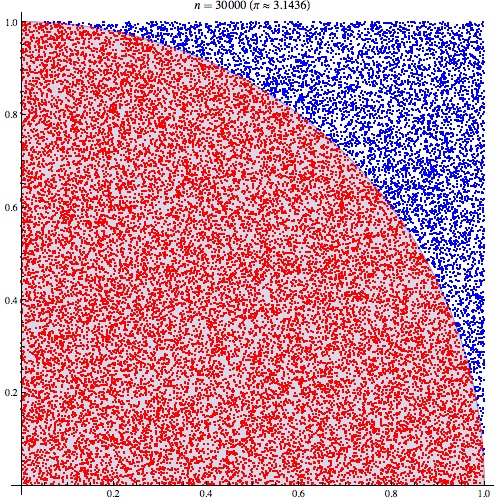
\includegraphics[width=0.35\textwidth]{figures/mc/pi}
	\caption{使用蒙特卡洛方法来计算$\pi$的值,这里使用30000个随机点,其$\pi$的估计值的误差范围在0.07\%以内(图片来自Wikipedia[CaitlinJo])}
	\label{f:mc-pi}
\end{figure}

蒙特卡洛方法的起源可以上溯到18世纪,法国数学家蒲丰为了验证大数定律,提出使用随机投针实验来估算圆周率$\pi$的值,该实验初步演示了蒙特卡洛方法的随机采样和统计估计的模拟思想。然而由于缺乏高速计算工具,没有现代电子计算机,不可能进行千百万次的模拟计算,由于技术条件不成熟,蒙特卡洛方法经历了近两个世纪漫长的启蒙时期。

现代形式的蒙特卡洛方法最早是由斯塔尼斯拉夫·乌拉姆(Stanislaw Ulam)于20世纪40年代晚期,在洛斯阿拉莫斯国家实验室进行核武器研究时提出,当时在核武器的研制过程中涉及中子在结构复杂的原子弹内扩散和增值的问题,需要求解高维玻尔兹曼方程,这是一个高维偏微分积分方程,无法使用解析方法求解;跟随着乌拉姆的突破性工作,计算机科学家约翰·冯·诺伊曼(John von Neumann)立即明白了它的重要意义,并把它编程实现在世界上第一台电子计算机ENIAC上;随后于1953年,尼古拉斯·梅特罗波利斯(Nicholas Metropolis)与其他四位科学家提出了著名的梅特罗波利斯算法\cite{a:EquationofStateCalculationsbyFastComputingMachines},该算法对近代工业和科技发展产生了非常重要的影响,其甚至被称为20世纪最重要的算法。

蒙特卡洛方法被广泛运用于现代科技和工业中,它主要被应用于最优化理论,数值积分方法以及从概率分布函数中产生随机数等领域和方面。在计算机图形学中,蒙特卡洛方法主要被应用于物理模拟以及光照传输中的积分运算,从后面第\ref{chp:path-tracing}章即将介绍的渲染方程的路径积分形式中可以看到,其被积函数是一个具有无限维度的高维函数,在离线渲染领域,渲染方程几乎只能使用蒙特卡洛方法来进行计算。

本章首先复习概率论相关的一些基础知识和概念,例如随机变量,方差,数学期望等,然后由大数定律推导出蒙特卡洛积分形式;紧接着讨论怎样对已知分布函数进行随机数取样,这包括逆变换算法,取舍算法,复合算法以及基于马尔可夫链(Markov Chain)\mathindex{马尔可夫链}{Markov Chain}的梅特罗波利斯算法(Metropolis algorithm)\mathindex{梅特罗波利斯算法}{Metropolis algorithm};由于蒙特卡洛方法都存在一定范围的误差,所以最后我们讨论一些有效的减少蒙特卡洛模拟方差的方法,例如重要性采样,以及基于数论的拟蒙特卡洛方法(Quasi-Monte Carlo method)\mathindex{拟蒙特卡洛方法}{Quasi-Monte Carlo method}等。本章讨论的内容是后面路径追踪,光子映射等全局光照算法的重要基础知识和工具。




\section{概率论基础}\label{sec:mc-probability}
自然界中的很多现象或事件,在一定的范围之内是随机发生的,称为随机事件(random events)\mathindex{随机事件}{random events}。然而经过人们的观察,在这些事件的大量重复的过程中,它们的分布却呈现出某种规律性,例如股票的波动,人口统计中的一些特性,骰子分布等等。因此,统计学就是一门通过对大量采样样本进行统计以计算出其分布规律的学科。而既然随机事件在大量重复试验下服从一定的分布,那么如果我们已知某随机事件服从某一分布,就可以通过大量重复试验来计算该随机事件的某些特征,例如统计平均值。这样就可以使用随机的方法来解决确定性的问题。



\subsection{随机变量}
为了利用随机性来解决数学问题,首先需要使用数学语言来描述随机事件。在数学中,随机事件用随机变量(random variables)\mathindex{随机变量}{random variables}来表示,随机变量用大写字母表示,例如$X$。随机变量是一个函数,它将某一集合内的随机事件(或者另一个随机变量)映射到一个数值的集合,或者通俗地说,随机变量$X$用一个数值来表述一个随机事件,例如用1,2,3,4,5和6这六个数值来表述骰子的六个可能的随机事件,这样就可以用数学方法来描述随机事件。随机变量的值用小写字母表示,例如$x$,称为随机数(random numbers)\mathindex{随机数}{random numbers}。随机变量的输入集合也可以是另一个随机变量,这时我们将服从一种分布的随机变量转换为服从另一种分布的随机变量\footnote{注意:一个随机变量的值是某个随机事件的数学表示,当我们看到一个随机变量时,它不是一个普通的数字,我们应该要联系到它背后的随机事件,例如对于骰子,随机变量的值6表示的是某一次骰子记录的结果为数字为6的那一面朝上。所以我们说随机变量始终是一个“映射”或“函数”,但是仅有将一个基本的随机变量(如$X$)转换为了一个分布的随机变量(如$Y$)时,才能写成函数的形式,对于基本随机变量$X$,它仅表示一种映射。},例如:$Y=f(X)$。

随机变量$X$的每个值$x$都关联着一个概率,即每次采样时该值(或对应随机事件)出现的概率,随机变量所有可能值组成的概率分布函数称为概率密度函数(probability density function,PDF)\mathindex{概率密度函数}{probability density function},用$p$表示,如图\ref{f:mc-cdf}(a)所示。

\begin{figure}
	\sidecaption
	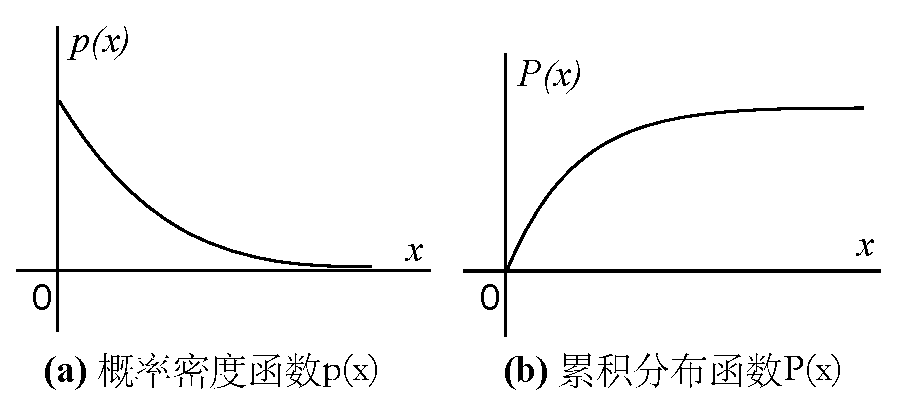
\includegraphics[width=0.6\textwidth]{figures/mc/cdf}
	\caption{概率密度函数p(x)表示随机采样结果处于$[x,x+dx]$区间的概率,相应地,累积分布函数则是采样的结果处于$(-\infty,x]$区间内的概率}
	\label{f:mc-cdf}
\end{figure}

随机变量可以是离散或连续的,例如骰子游戏,每次扔骰子的结果被映射为一个离散的随机变量的值$x_i$,所有值的集合为$X=\{1,2,3,4,5,6\}$,第$i$个随机数值出现的概率为$p_i=1/6$。对于离散随机变量,每个随机数对应的概率满足:$0\leq p_i \leq 1$,所有离散变量的概率之和满足:$\sum_i p_i=1$。

对于连续随机变量$X$,其概率密度函数$p(x)$是通过落于$x$附近的区间$[x,x+dx]$内的随机数的概率$p(x)dx$来定义的,然而这种定义方式并不直观,所以连续随机变量的概率分布一般通过更直观的称为累积分布函数(cumulative distribution function,CDF)\mathindex{累积分布函数来定义}{cumulative distribution function}来定义,连续随机变量$X$的累积分布函数用大写字母$P$表示,其定义为:

\begin{equation}
	P(y)=Pr\{x\leq y\}={\rm \int}_{-\infty}^{y}p(x){\rm d}x
\end{equation}

累积分布函数$P(y)$定义的是所有随机数的值中小于或等于$y$的随机变量的概率的积分\footnote{注意这里我们使用两种形式来表示累积分布函数,$P(y)$所代表的变量形式,以及$Pr\{x\leq y \}$所代表的范围的形式。},所以累积分布函数是一个递增函数,如图\ref{f:mc-cdf}(b)所示。连续随机变量的概率密度函数$p(x)$具有以下属性:

\begin{equation}\label{eq:mc-continuous-pdf}
	\begin{aligned}
		\forall x: p(x)&\geq 0\\
		{\rm \int}_{-\infty}^{+\infty}p(x){\rm d}x&=1\\
		p(x)&= \cfrac{{\rm d}P(x)}{{\rm d}x}
	\end{aligned}
\end{equation}

\noindent 相应地,随机变量的值$x$落于区间$[a,b]$的概率为:

\begin{equation}
	\begin{aligned}
		Pr\{a\leq x\leq b\}&=Pr\{x\leq b\}-Pr\{x\leq a\}\\
		&=P(b)-P(a)={\rm \int}_{a}^{b}p(z){\rm d}z
	\end{aligned}
\end{equation} 

例如对于如图\ref{f:mc-cdf}(b)所示的累积分布函数$P(x)=1-\mathrm{e}^{-x},x\in[0,\infty)$,它对应的概率密度函数为$p(x)=P(x)^{'}=\mathrm{e}^{-x},x\in[0,\infty)$,如图\ref{f:mc-cdf}(a)所示。

特别地,对于$[a,b]$区间上的均匀分布,其概率密度函数为常数$ \cfrac{1}{b-a}$,它表示随机采样结果落于区间$[x,x+dx]$的概率在每个$x$处都相同,如图\ref{f:mc-uniform-cdf}所示。均匀分布的随机变量是整个蒙特卡洛方法的基础,在计算机模拟中,通常都是由系统提供的${\rm random}()$函数生成某个区间内的均匀分布,然后使用后面讲述的方法将均匀分布的随机变量转换为具有任意概率密度分布的随机变量。

\begin{figure}
\sidecaption
		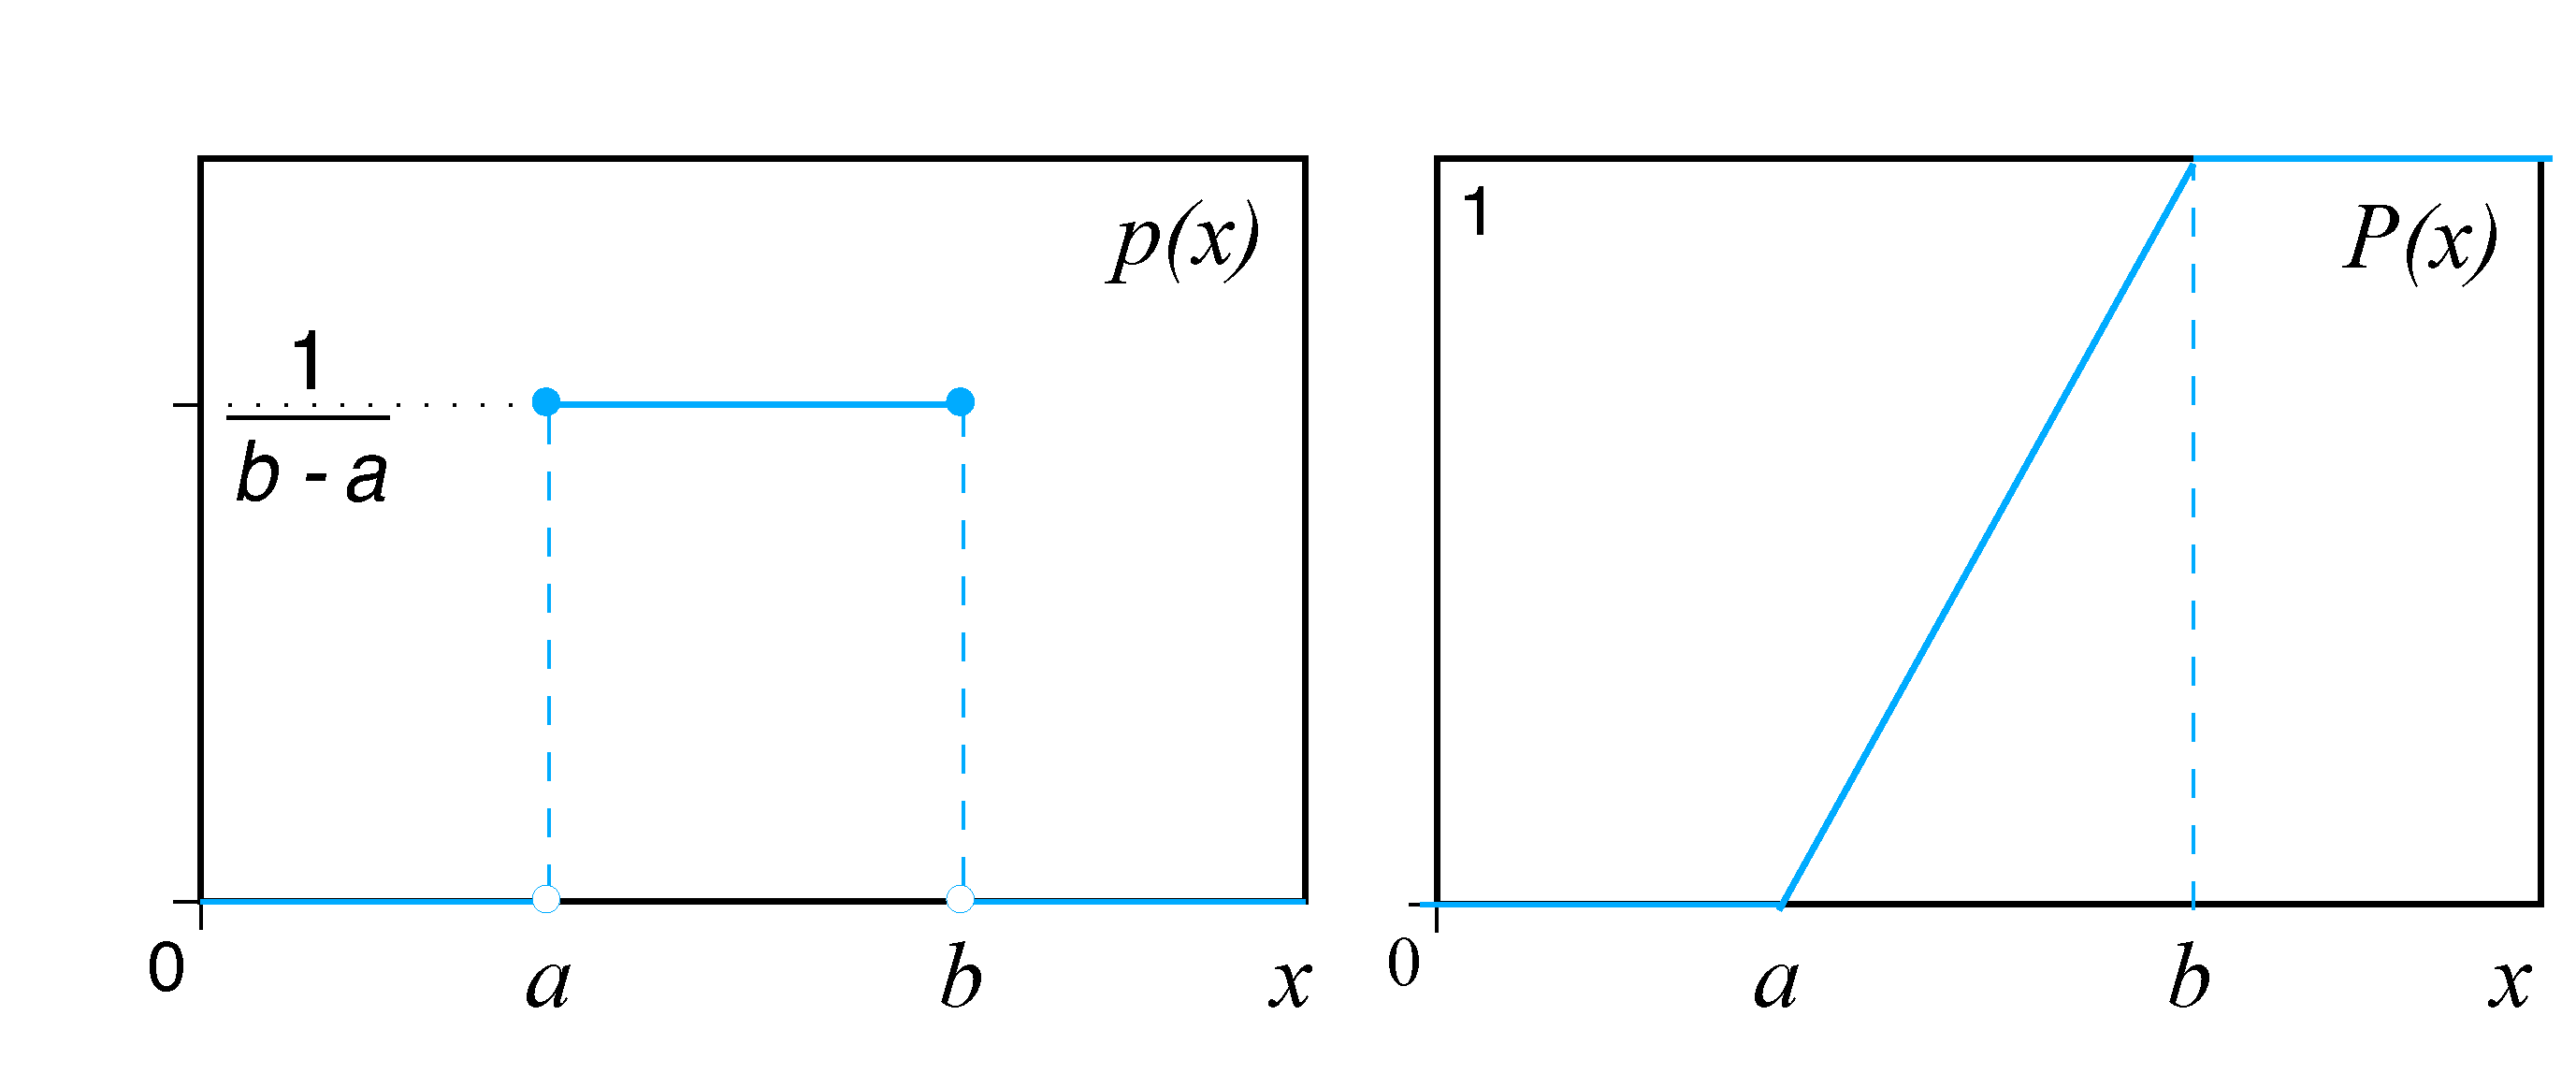
\includegraphics[width=0.65\textwidth]{figures/mc/uniform-cdf}
	\caption{均匀分布是最基础的随机变量,它的概率密度函数$p(x)$是一个常数}
	\label{f:mc-uniform-cdf}
\end{figure}




\subsection{期望与方差}
随机变量的概率密度函数和累积分布函数能够完整地描述一个随机变量的特征,但单个随机变量具有随机性,它对于实际的数学分析并没有什么意义,我们对多个随机变量采样的统计结果更感兴趣,本节介绍对随机函数进行多次采样结果(而不是单个随机变量)的一些数字特征,例如期望,方差及相关系数。

对于离散随机变量$X$,假设其值$x_i$对应的采样概率为$p_i$,则该随机变量$X$的数学期望(expected value)\mathindex{数学期望}{expected value},又称为均值(mean)\mathindex{均值}{mean},为:

\begin{equation}\label{eq:mc-expected-value}
	E[X]=\sum_{i=1}^{n}p_i x_i
\end{equation} 

期望代表的是对一个随机变量$X$进行采样的平均结果。例如对于骰子的例子,它的数学期望为:

\begin{equation}
	\begin{aligned}
		E[X_{\rm die}]&=\sum_{i=1}^{6}p_i x_i\\
		&=\sum_{i=1}^{6} \cfrac{1}{6}x_i = \cfrac{1}{6}(1+2+3+4+5+6)\\
		&=3.5
	\end{aligned}
\end{equation}

对应地,对于连续随机变量$x$,其期望为随机变量值$x$与其概率密度函数$p(x)$的乘积在全定义域上的积分(如果该积分绝对收敛):

\begin{equation}\label{eq:mc-continuous-e}
	E[X]={\rm \int}_{-\infty}^{+\infty}xp(x){\rm d}x
\end{equation}

上述的关于随机变量的期望的定义在概念上很好理解,但是通常我们对随机变量的函数更感兴趣,考虑随机变量$Y=g(X)$,并且只知道随机变量$X$的概率分布,怎样求出随机变量$Y$的期望呢?

随机变量函数的数学期望可以通过下面的定理来求,即无意识的统计规律
(law of the unconscious statistician)\mathindex{无意识的统计规律}{law of the unconscious statistician}: 设$Y$是随机变量$X$的函数:$Y=g(X)$,这里$g$是连续函数,如果$X$是离散型随机变量,它的概率分布为$P\{X=x_i\}=p_i,i=1,2,\cdots$,若$\sum^{\infty}_{i=1}g(x_i)p_i$绝对收敛, 则有:

\begin{equation}
	E[Y]=E[g(X)]=\sum^{\infty}_{i=1}g(x_i)p_i
\end{equation}

如果$X$是连续型随机变量,它的概率密度为$p(x)$,若${\rm \int}^{\infty}_{-\infty}g(x)p(x){\rm d}x$绝对收敛,则有:

\begin{equation}
	E[Y]=E[g(X)]={\rm \int}^{\infty}_{-\infty}g(x)p(x){\rm d}x
\end{equation}

该定理的重要意义在于,当求$E[Y]$时,我们不必算出$Y$的分布律或概率密度,而只需要利用$X$的分布律或概率密度就可以了。

除了均值,我们需要知道这些随机变量的采样结果相对其期望的偏离程度,这可以用每个随机变量与期望值差的期望的绝对值来表示,即:$|E[x-E[X]]|$,由于涉及绝对值不便于计算,所以使用该期望的平方来表征该量,即方差(variance)\mathindex{方差}{variance}$\sigma^2$, 表示为$V\{X\}$,方差的平方根$\sigma$称为标准差(standard deviation)\mathindex{标准差}{standard deviation}。对于离散随机变量,其方差为:

\begin{equation}
	\sigma^2=E[(x-E[X])^2]=\sum_i (x_i-E[x])^2p_i
\end{equation}

\noindent 对于连续随机变量,其方差为:

\begin{equation}\label{e:discrete-variance}
	\sigma^2=E[(x-E[x])^2]={\rm \int} (x-E[x])^2 p(x){\rm d}x
\end{equation}

方差具有以下性质:
\begin{enumerate}
	\item 若$C$是常数,则:$V\{C\}=0$
	\item 若$C$是常数,$X$为随机变量,则:$V\{CX\}=C^2V\{X\}$
	\item 若$X$和$Y$是两个独立的随机变量,则:$V\{X+Y\}=V\{X\}+V\{Y\}$
\end{enumerate}



\subsection{大数定律}
在统计学中,很多问题涉及对大量独立的随机变量采样$x_i$的和进行处理,这些随机变量拥有相同的概率密度函数$p$,这样的随机变量称为独立同分布(independent identically distributed,IID)\mathindex{独立同分布}{independent identically distributed}的随机变量,例如在实验条件保持不变的情况下,一系列抛硬币的正反面结果就是独立同分布的。当这些随机变量采样的和被除以这些随机变量采样的数量$N$时,我们得到该随机变量的期望的一个估计(estimator)\mathindex{估计}{estimator},即:

\begin{equation}
	E[X]\approx\overline{X}=  \cfrac{1}{N}\sum_{i=1}^{N}x_i
\end{equation}

\begin{myshaded}
	所谓估计的概念,可以理解为是对应数学模型的一种具体的(往往是近似的)求解方法,比如在这里随机变量的数学期望模型为$E[X]=\sum^{n}_{i=1}p_ix_i$(对于离散随机变量),或者$E[X]=\int xp(x){\rm d}x$(对于连续随机变量),上述的随机变量的期望应该怎么求解呢?我们可以对该随机变量重复$N$次采样,这形成一些独立同分布的随机数,然后通过对这些随机数进行统计计数来近似上述的期望模型,即使用估计$\overline{X}=  \cfrac{1}{N}\sum_{i=1}^{N}x_i$来近似$E[X]$。
\end{myshaded}

随着随机采样数量$N$的增大,该估计的方差逐渐减小。我们希望$N$值足够大,以至于该估计的值能够充分接近期望的值,这样我们能够将统计方法用于解决确定性问题。大数定律(law of large numbers)\mathindex{大数定律}{law of large numbers}告诉我们,当$N\rightarrow\infty$时,我们可以确定随机变量的统计平均值趋近于期望的值,即:

\begin{equation}\label{eq:mc-large-numbers}
	P\Bigg\{ E[X]=\lim_{N \to \infty} \cfrac{1}{N}\sum_{i=1}^{N}x_i \Bigg\}=1
\end{equation} 

大数定律告诉我们,随机变量的期望描述的加和(如式\ref{eq:mc-expected-value})或积分(如式\ref{eq:mc-continuous-e})计算,可以通过对随机变量执行大量的重复采样,这得到一些独立同分布的随机数,然后使用这些采样结果的统计平均来近似。

大数定律是蒙特卡洛方法的重要基础,关于大数定律的证明过程可以参见切比雪夫不等式以及中心极限定理,这里不再对其进行详述,我们只需要理解通过对某个分布函数执行大量重复采样来近似随机数期望这种思路即可。




\section{蒙特卡洛积分}
设想我们要计算一个一维函数的积分,例如${\rm \int}_a^{b}f(x){\rm d}x$,数值分析方法通常使用一些近似方法来计算积分,最简单的求积分的方法便是将被积函数沿作用域上划分成多个区域,然后计算这些区域面积的和。如果这些区域的划分在作用域上是均匀的,如图\ref{f:mc-quadrature-rules}所示,则对积分$I$的近似可以写成:

\begin{equation}\label{eq:mc-quadrature-rules}
	\begin{aligned}
		I&={\rm \int}_{a}^{b}f(x){\rm d}x \\
		&\approx \sum_{i=1}^{N}f(x_i) \cfrac{(b-a)}{N}
	\end{aligned}
\end{equation}

\noindent 这里$f(x_i)$是每个区间的中点位置的函数值,$N$越大,则该近似越逼近积分$I$的真实结果。

\begin{figure}
\sidecaption
	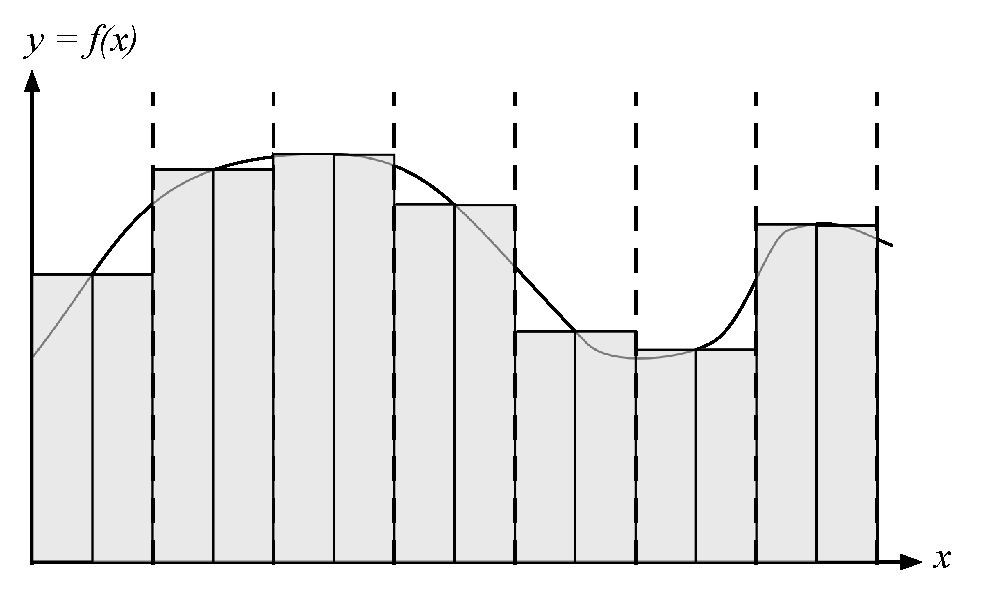
\includegraphics[width=0.55\textwidth]{figures/mc/mc-finite-integration}
	\caption{确定性的一维积分}
	\label{f:mc-quadrature-rules}
\end{figure} 

当我们尝试将这种确定性的积分方法推广到$d-$维积分的时候,它要求将原始函数分为$N^d$个采样空间,显然这种方法不适合用于多维积分的计算。当然也存在一些其它的计算多维积分的方法, 但是其中在计算机图形学领域用的最多的还是蒙特卡洛方法,蒙特卡洛方法有很多种不同的用途,其中最重要的一种就是用于计算高维积分。

在推导具体的蒙特卡洛估计之前,我们首先需要了解一下蒙特卡洛方法和传统数值分析方法的区别。式\ref{eq:mc-quadrature-rules}和式\ref{eq:mc-large-numbers}虽然看起来具有比较相似的思路:即它们都是计算$N$个“采样点”的平均值,但是前者是一种传统的数值近似方法,它必须在每个维度上使用同样的近似结构(即对每个维度执行空间划分),因此它的采样的数量是和维度相关的;而大数定律的采样点来自于满足某个分布的一个随机数,这个随机数直接对一维或多维空间进行采样,这个采样的数量与函数的维度并无直接关系。

大数定律用于对期望表示的积分形式进行估计,即对积分${\rm \int}_{-\infty}^{\infty}xf(x){\rm d}x$进行估计,但是我们通常需要求得一个任意函数的积分,假设函数$g(x)$的定义域为$x\in S$($S$可以是一个多维空间,此时$x$表示一个向量),我们希望计算以下积分:

\begin{equation}
	I={\rm \int}_{x\in S}g(x){\rm d}\mu
\end{equation}

根据前面的描述,给定任意一个实数函数$f$以及一个随机变量$x\sim p(x)$,我们可以使用以下的一个和的公式来近似$f(x)$的期望:

\begin{equation}\label{e:sum}
	E[f(x)]={\rm \int}_{x\in S}f(x)p(x){\rm d}\mu\approx \cfrac{1}{N}\sum_{i=1}^{N}f(x_i)
\end{equation}

这个结果就是使用蒙特卡洛方法求积分的核心思想,因为期望表示的积分可以使用多个随机数采样值的和的形式来近似。对\ref{e:sum}稍作变换, 使用$g=fp$ 代替被积函数,则上式变为:

\begin{equation}
	{\rm \int}_{x\in S}g(x){\rm d}\mu\approx \cfrac{1}{N}\sum_{i=1}^{N} \cfrac{g(x_i)}{p(x_i)}
\end{equation}

\noindent 对于该公式,$p$必须为正,我们定义$I$的估计(estimator)为$I_N$,即:

\begin{equation}\label{eq:mc-mc-extimator}
	I_N= \cfrac{1}{N}\sum_{i=1}^{N} \cfrac{g(x_i)}{p(x_i)}
\end{equation}

\noindent 该估计的期望值为:

\begin{equation}
	\begin{aligned}
		E[I_N]&=E[ \cfrac{1}{N}\sum_{i=1}^{N} \cfrac{g(x_i)}{p(x_i)}]\\
		&= \cfrac{1}{N}\sum_{i=1}^{N}E[ \cfrac{g(x_i)}{p(x_i)}]\\
		&= \cfrac{1}{N}N{\rm \int}  \cfrac{g(x)}{p(x)}p(x){\rm d}x\\
		&={\rm \int} g(x){\rm d}x\\
		&=I
	\end{aligned}
\end{equation}

\noindent 由此可以看出该估计可以用于用作$I$的近似,该估计的方差为:

\begin{equation}\label{e:variance}
	\sigma^2= \cfrac{1}{N}{\rm \int}( \cfrac{g(x)}{p(x)}-I)^2p(x){\rm d}x
\end{equation}

由此可以看出,随着$N$的增加,其方差随着$N$线性降低,由于估计的误差正比于其标准差$\sigma$,因此估计的误差随着$\sqrt{N}$线性降低。这就是一般蒙特卡洛方法的特点,实际上蒙特卡洛方法最大的问题就是估计逼近正确结果的速度非常慢,例如需要使用四倍多的采样点才可以仅仅减少一半的误差。 

理论上,$p(x)$的选择可以是任意的,这也是蒙特卡洛方法的一大优点,因为通常很难生成与被积函数具有一致分布的随机数。但是从式\ref{eq:mc-mc-extimator}也可以看出,通过使$g(x_i)$和$p(x_i)$的比值尽可能地小也可以减少估计误差,在实践上这通常使$p(x)$的分布接近于$g(x)$,这称为本章后面会讨论的重要性采样的基础。

终上所述,蒙特卡洛方法是一种非常简单而强大,可以近似计算任意函数积分的数值方法。蒙特卡洛方法可以归纳为以下步骤:

\begin{itemize}
	\item 首先对一个满足某种概率分布的随机数进行采样。
	\item 使用该采样值计算$ \cfrac{g_i}{p(x_i)}$的值,这称为该样本的贡献值。
	\item 最后对所有采样点计算的结果求平均值。
\end{itemize}

在这些步骤中,最困难的部分涉及怎样对一个任意分布函数进行采样,我们将在第\ref{sec:Sampling-Random-Variables}节讨论一些常用的采样方法;其次,蒙特卡洛方法的另一个重要内容是涉及怎样减少方差,第 \ref{sec:Variance-Reduction}节将会讨论这方面的内容。





\section{对分布$p(x)$进行采样}\label{sec:Sampling-Random-Variables}
由上节的内容可知,蒙特卡洛方法涉及两个基本的步骤:采样和求平均值,本节就讨论几种不同采样方法。

首先我们定义什么是采样,考虑一个定义域空间$\Omega_0$以及一个概率密度函数$p(x)$,其中$x\in\Omega_0$,满足:

\begin{equation}
	{\rm \int}_{\Omega_0}p(x){\rm d}x=1
\end{equation}

采样的过程是这样一个算法,它能够从$p(x)$对应的随机变量$X$中产生一系列随机数$X_1,X_2,...$,使对于任意$\Omega\in\Omega_0$满足:

\begin{equation}
	P\{X_k\in\Omega\}={\rm \int}_{\Omega}p(x){\rm d}x\leq 1
\end{equation}

实际上我们不能直接从$p(x)$产生随机数,在计算机程序中这个过程必须要求首先具有某些基础随机数的一个序列。我们可以借助计算机操作系统提供的${\rm random}(u)$函数来产生一个均匀分布的随机数,又称为伪随机数(pseudorandom numbers)\myindex{伪随机数}{pseudorandom numbers}, 定义这些随机数的值为$\xi_1,\xi_2,\cdots$,它们可以用来作为采样所需的基础随机数。




\subsection{逆变换算法}\label{sec:mc-inversion-method}
逆变换算法是1947年由乌拉姆提出的,它的定义如下:设$X$是连续随机变量,其累计分布函数为$P_X$,如果随机变量$Y$是一个$[0,1]$上的均匀分布,则随机变量$P^{-1}_X(Y)$具有和$X$一样的概率分布。

逆变换算法的直观解释可以由图\ref{f:mc-inversion-method}得出,图中$dy$表示的随机变量是[0,1]上的均匀分布,由式\ref{eq:mc-continuous-pdf}可知,随机变量$X$中的值落于${\rm d}x$区间的概率$p(x)= \cfrac{{\rm d}P(x)}{{\rm d}x}= \cfrac{{\rm d}y}{{\rm d}x}$,所以$Y$上的均匀分布被映射到满足$p(x)$的随机变量$X$上。

\begin{figure}
	\sidecaption
	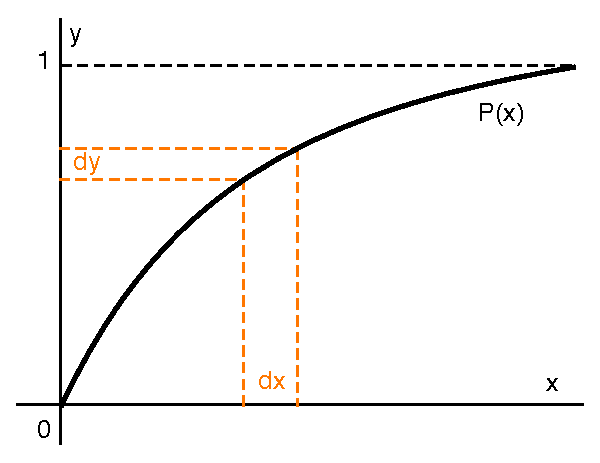
\includegraphics[width=0.5\textwidth]{figures/mc/inversion-method}
	\caption{逆变换算法将一个满足[0,1]上的均匀分布的随机变量$Y$,通过$X=P^{-1}(Y)$映射到满足概率分布$p(x)$的随机变量$X$上}
	\label{f:mc-inversion-method}
\end{figure}

以下我们以一个离散分布的例子来进一步解释逆向变换算法的过程,设一个离散随机变量具有4个可能的值,其对应的概率分别为:$p_1,p_2,p_3$和$p_4$ ,这些概率满足:$\sum_{i=1}^{4}p_i=1$, 该随机变量对应的概率密度函数如图\ref{f:simple-pdf}所示。

\begin{figure}
\sidecaption
	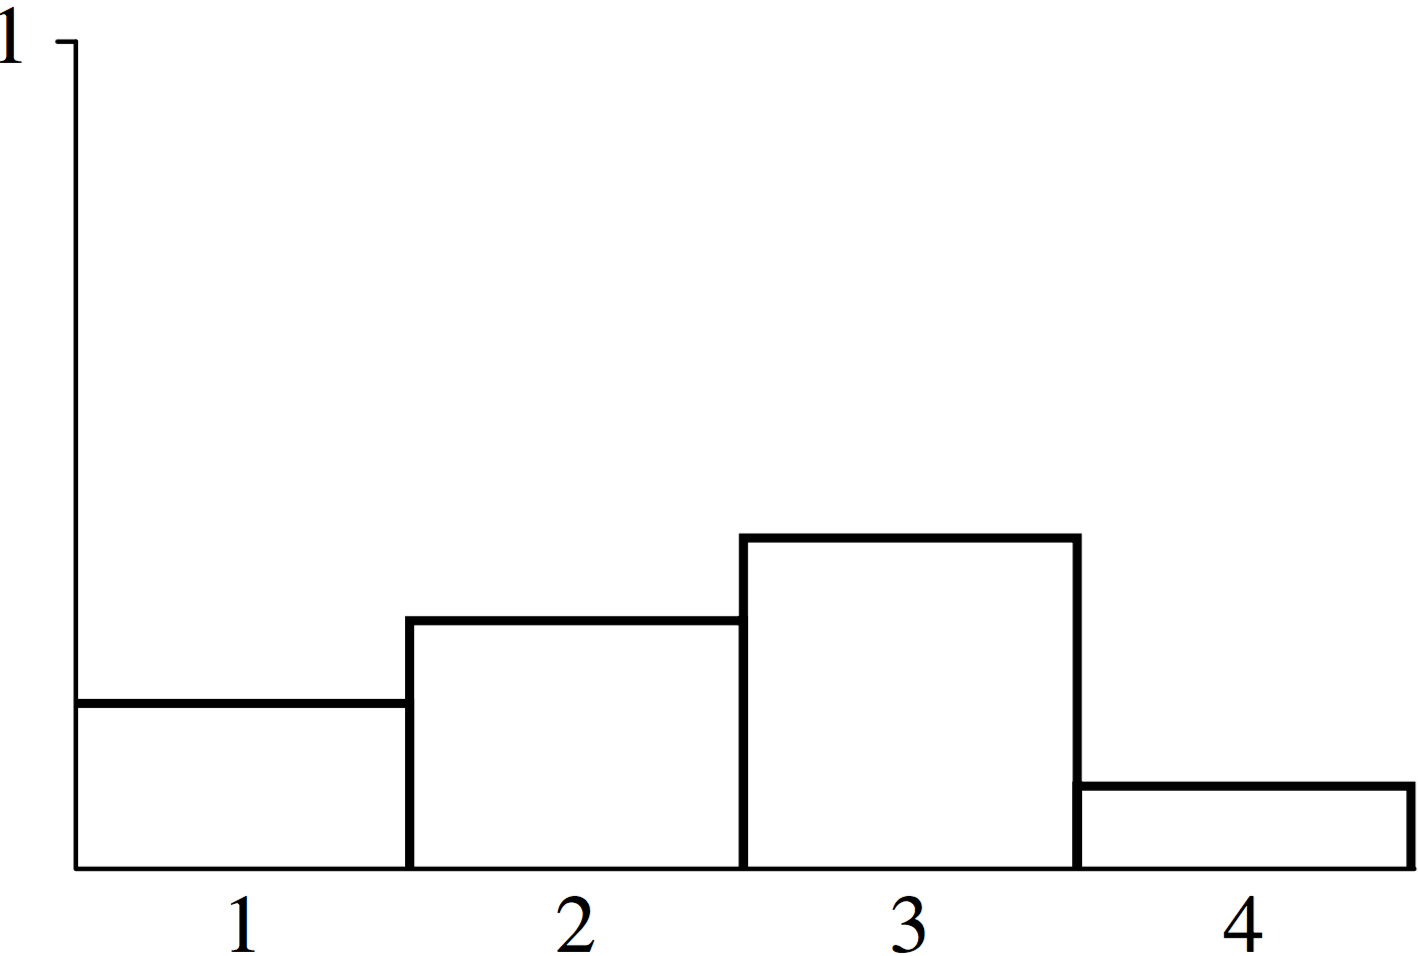
\includegraphics[width=0.45\textwidth]{figures/mc/mc-3}
	\caption{一个具有4个输入事件的离散随机变量的概率密度分布,每个随机数$x_i$的概率为$p_i$}
	\label{f:simple-pdf}
\end{figure}

为了使用逆变换算法从一个任意分布中进行采样,首先需要求出其对应的累积分布函数
$P(x)$,对于连续随机变量,$P$是$p$在全定义域上的积分,对于离散随机变量,可以使用前$i$个$p$的值的和作为$P(x_i)$的值,如图\ref{f:mc-discrete-cdf}所示。注意,为了满足所有随机事件的概率之和为1,最右边的条的高度应该为1。

\begin{figure}
\sidecaption
	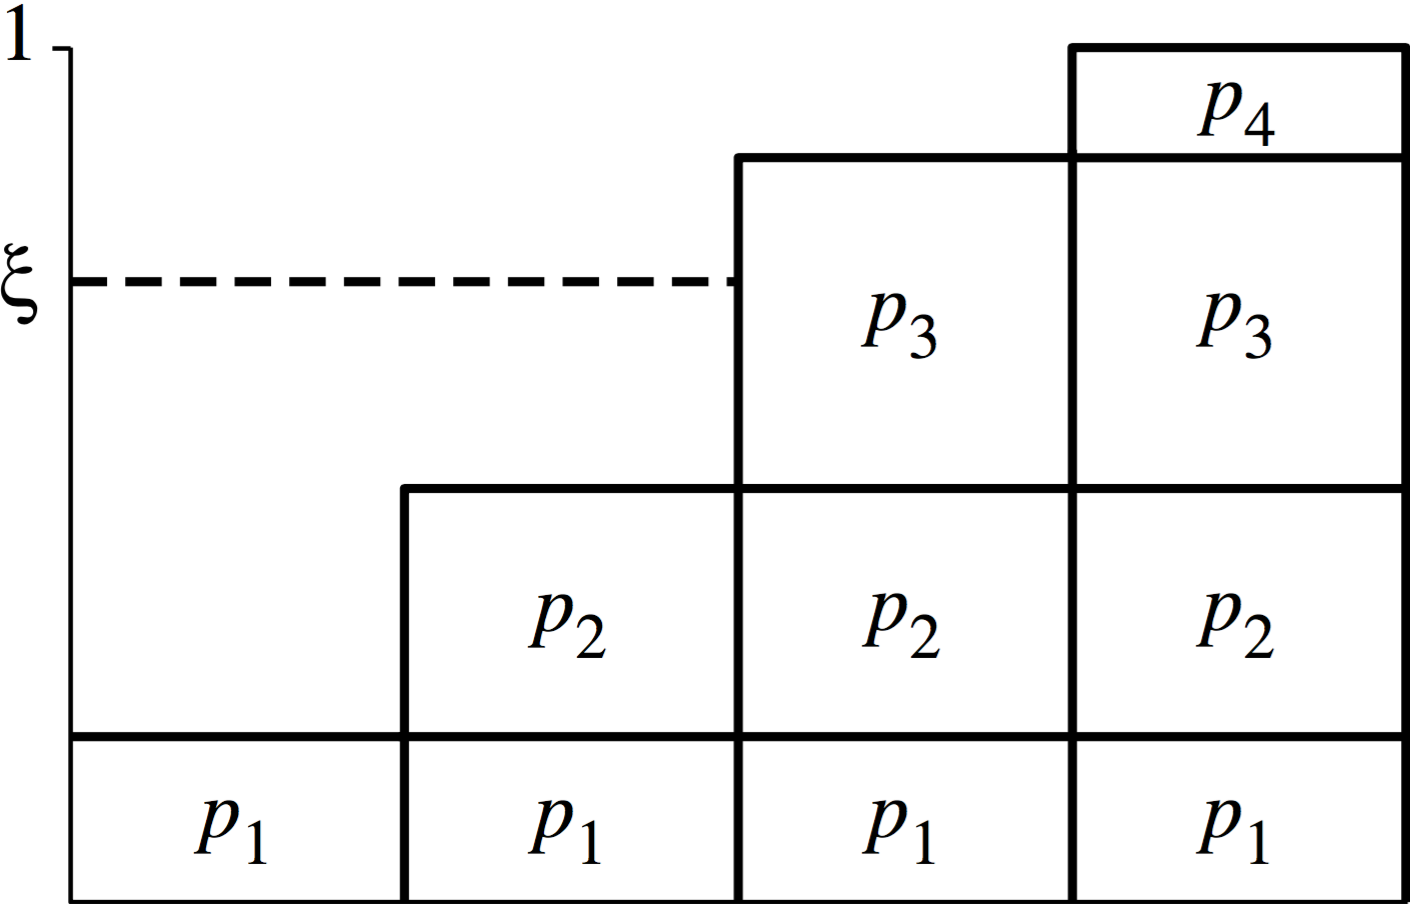
\includegraphics[width=0.45\textwidth]{figures/mc/mc-4}
	\caption{从离散随机变量的概率密度函数$p$构建概率分布函数$P$的过程,$[0,1]$上均匀分布的随机数$\xi$被按照概率分布映射到离散随机变量$X$上}
	\label{f:mc-discrete-cdf}
\end{figure}

在图\ref{f:mc-discrete-cdf}中,一个标准的$[0,1]$上的均匀分布的随机变量分布在纵坐标上,通过在水平方向上延伸$\xi$可以和具有概率$p_i$的第$i$个输入事件相交,因为$\xi$是服从均匀分布的,所以具有更大概率的$p_3$比$p_4$拥有更多的机会被选择,所以通过这样的方式,$[0,1]$上的均匀分布$\xi$被完全变换为服从概率密度函数$p(x)$的离散随机变量$X$。

通过上述的示例,我们可以推导出使用逆变换算法从一个概率密度函数$p(x)$产生随机数$X_i$的步骤:

\begin{enumerate}
	\item 首先计算$p(x)$的累计分布函数:$P(x)={\rm \int}_{0}^{x}p(x^{'}){\rm d}x^{'}$。
	\item 其次计算累计分布函数的反函数:$P^{-1}(x)$。
	\item 然后从一个$[0,1]$上的均匀分布产生一个随机数$\xi$。
	\item 最后将随机数$\xi$代入$P(x)$的反函数求出满足$p(x)$分布的随机数:$X_i=P^{-1}(\xi)$。
\end{enumerate}




\subsection{取舍算法}\label{sec:mc-accept-reject}
在许多情况下,逆变换算法无法被使用:首先是某些累积分布函数无显式解析表达式,因此写不出反函数,例如某些概率密度函数没有边界,不能归一化;其次是反函数无显式表达式,因此解不出反函数;再次是在整个求累积分布函数和反函数的过程中,这里面可能涉及大量初等函数的计算,因此采样成本很高。

为了在计算机中对任意分布函数进行采样,冯·诺伊曼于1947年提出了取舍算法(acceptance-rejection method)\mathindex{取舍算法}{acceptance-rejection method},这种方法不需要对概率分布函数执行归一化,并且它通常只需要直接使用计算机系统提供的均匀分布的随机数$\xi$即可。

取舍算法的思路很简单,它和本章开头讲述的蒲丰投针(如图\ref{f:mc-pi}所示)实验的原理类似,考虑一个任意函数$f(x)$\footnote{注意,这里的$f(x)$实际上是一个分布函数,然后在取舍算法中它通常并不是归一化的,因此我们偏向于称其为更具广泛意义的函数$f(x)$而不是归一化的$p(x)$。}被限定在$[a,b]$区间,在此区间外的所有值均为0,如图\ref{f:mc-rejection-idea}所示。

\begin{figure}
\sidecaption
	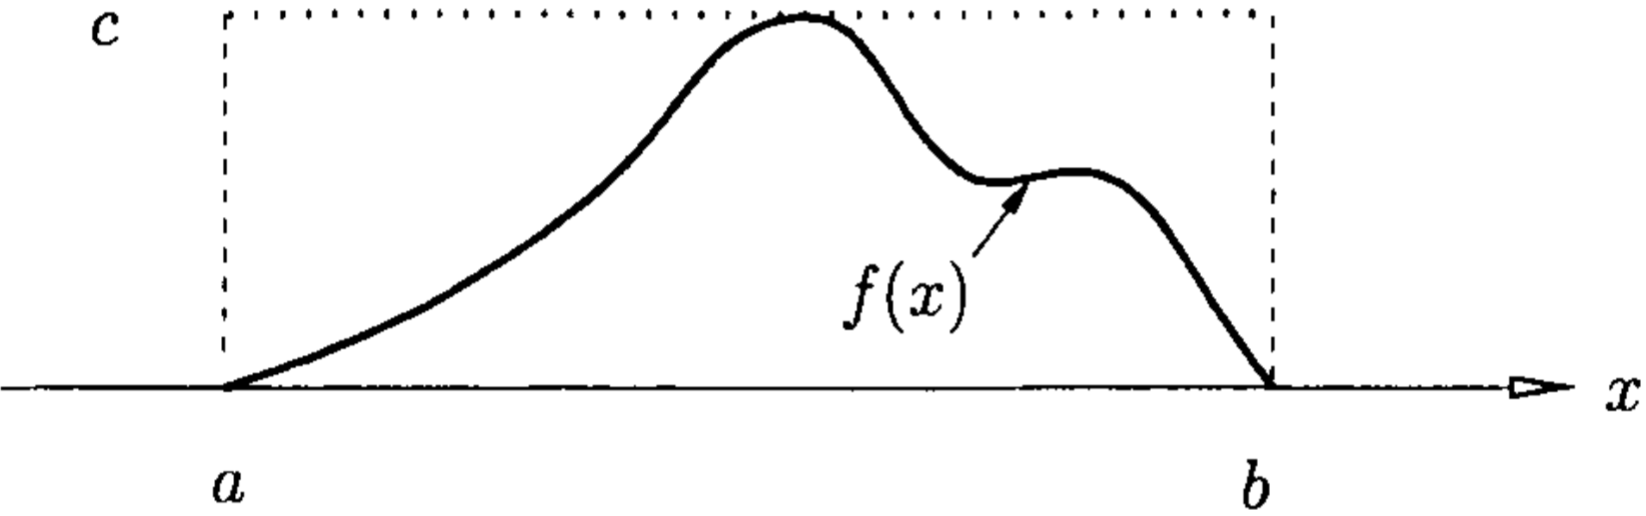
\includegraphics[width=0.65\textwidth]{figures/mc/mc-6}
	\caption{取舍算法在一个能够完全包围住$f(x)$的空间上均匀采样,然后选择(接受)处于函数$f(x)$范围内的采样值用来作为采样值,其他值则被抛弃(拒绝)}
	\label{f:mc-rejection-idea}
\end{figure}

在这种情况下产生一个随机变量$Y\sim f(x)$的过程非常直观,它可以被描述为以下接受-拒绝的过程:

\begin{enumerate}
	\item 产生一个$[a,b]$上均匀分布的随机数:$X\sim U(a,b)$。
	\item 产生一个$[0,c]$上独立于$X$的均匀分布的随机数:$Y\sim U(0,c)$($c$是函数$f(x)$的最大值)。 
	\item 如果$Y\leq f(X)$,则接受,接受的随机数为$Z=X$,否则$X$被拒绝,算法返回到第一步重新产生新的随机数。
\end{enumerate}

需要注意的是,每次采样产生的随机数矢量$(X,Y)$实际上是均匀地分布于一个矩形区域$[a,b]\times [0,c]$,因此被接受的随机数矢量$(X,Y)$则会均匀分布于函数$f(x)$以下的区域,这意味着被接受的随机数$X$服从概率分布$f(x)$。

\begin{figure}
\sidecaption
	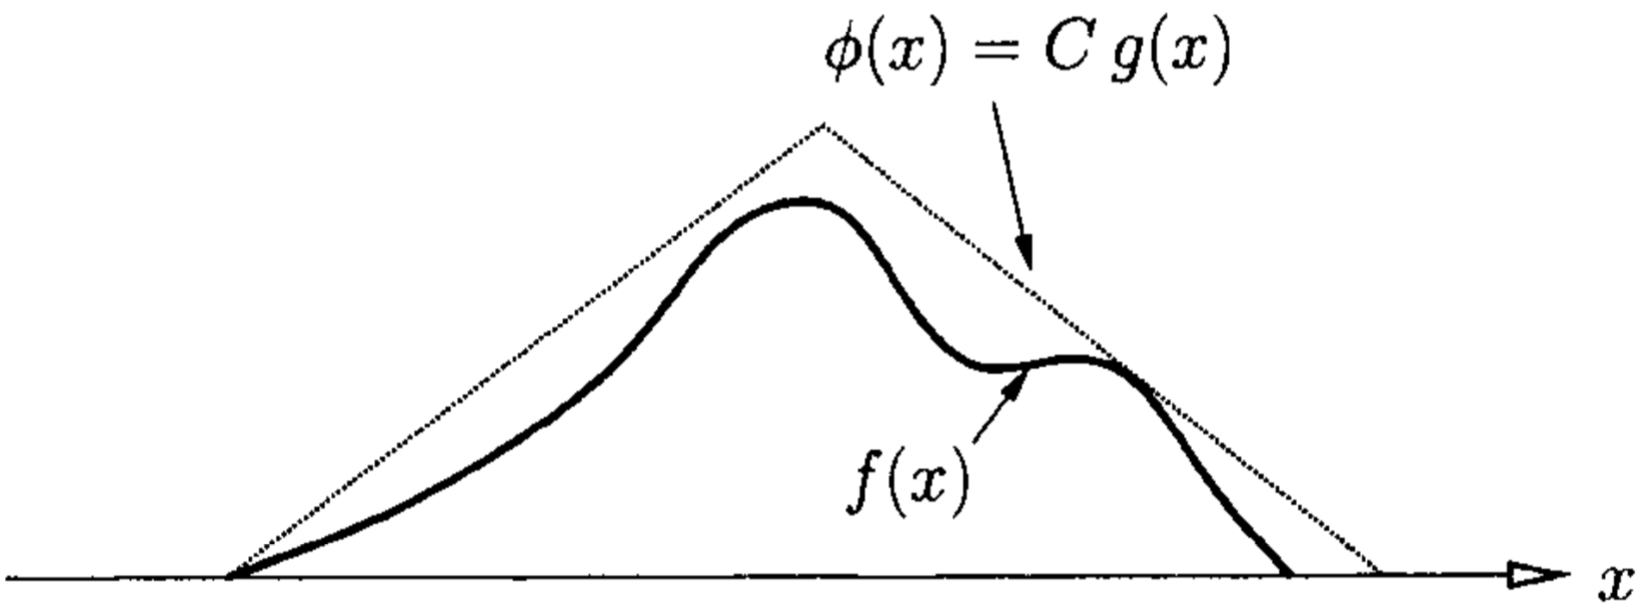
\includegraphics[width=0.65\textwidth]{figures/mc/mc-7}
	\caption{为了减少被拒绝的采样值的数量,使用一个接近$f(x)$而不是$c$的函数$\phi$来包围$f(x)$}
	\label{f:mc-rejection-generalized}
\end{figure}

取舍算法的缺点是其效率比较低,因为在接受一个随机数之前,大量的随机数被拒绝了。为了减少被拒绝的随机数的数量,实践上通常使用一个建议分布(proposal distribution)$\phi (x)=Cg(x)$来逼近$f(x)$(称为目标分布)的分布,其中$g(x)$是一个简单的函数,它通常能够比较容易的(例如使用逆向变换算法)产生随机数常数$C$用来保证$\phi (x)$能够完全覆盖$f(x)$,即:$\phi (x)\geq f(x)$,如图\ref{f:mc-rejection-generalized}所示。所以上述的取舍算法可以写为:

\begin{enumerate}
	\item 产生随机数:$X\sim g(x)$。
	\item 产生随机数:$Y\sim U(0,Cg(X))$。
	\item 如果$Y\leq f(X)$, 则接受随机数:$Z=X$,否则返回第一步。 
\end{enumerate}

取舍方法不需要对函数执行归一化,只需要找到一个能够覆盖该分布函数的更简单的分布(建议分布)即可,例如对于:

\begin{equation}
	f(x)= \cfrac{2}{\pi(1-x^2)^{ \frac{1}{2}}},0<x<1
\end{equation}

\noindent 可以使用更简单的建议分布函数:

\begin{equation}
	g(z)= \cfrac{1}{2(1-z)^{ \frac{1}{2}}}
\end{equation}

\noindent 注意,虽然对于一维的函数,取舍算法需要产生两个随机数来做取舍判断,但是由于它减少单次采样的计算成本,因此它和逆向变换算法仍然具有可比性。



\subsection{随机变量的变换}\label{sec:Transformation-of-Random-Variables}
在前面讨论逆向变换算法的时候,我们介绍了一种技术,它可以将一个满足均分分布的随机变量转换为一个满足任意分布的随机变量。本节,我们将讨论与之相关的一个更一般的问题:即将满足任意分布的一个随机变量转换为满足另一个分布的随机变量。

假设随机变量$X$的累积分布函数为$F_X(x)$,以及概率分布函数为$f_X(x)= \cfrac{{\rm d}F_X}{{\rm d}x}$,另一个随机变量$Y=y(X)$是关于$x$的连续单调递增函数,如图 \ref{f:transforming-function}(a)所示,我们的目标是求出$Y$的累积分布函数$F_Y(y)$的形式。

\begin{figure}
\sidecaption{
	\begin{subfigure}[b]{.35\textwidth}
		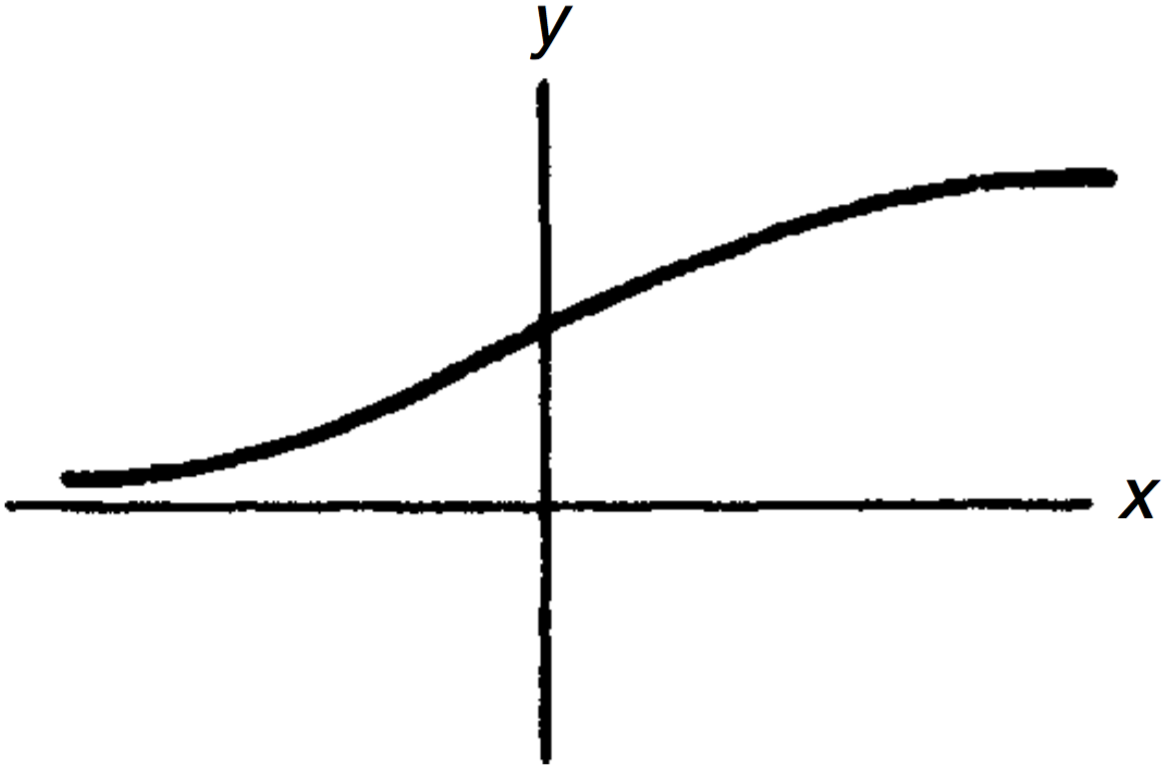
\includegraphics[width=1.\textwidth]{graphics/gi/mc-8}
		\caption{单调递增}
	\end{subfigure}
	\begin{subfigure}[b]{.28\textwidth}
		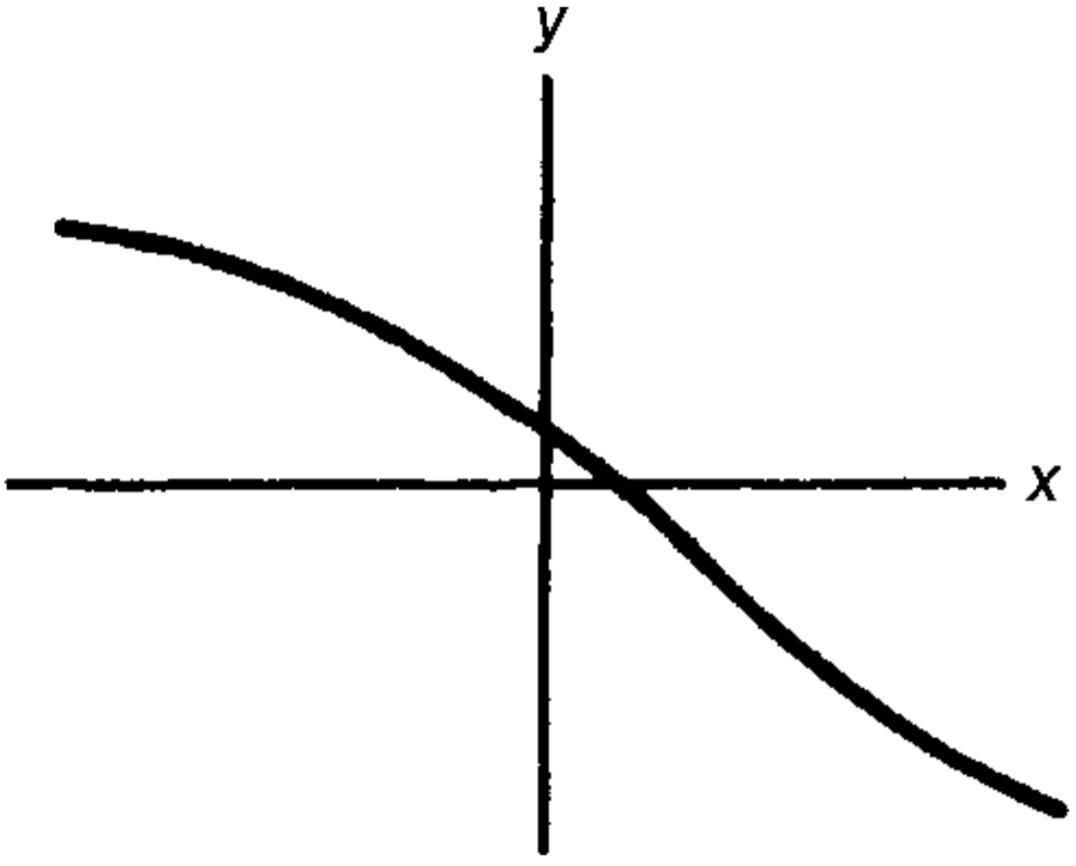
\includegraphics[width=1.\textwidth]{graphics/gi/mc-9}
		\caption{单调递减}
	\end{subfigure}}
	\caption{$y$是一个连续函数,其中(a)是关于$x$的单调递增函数,(b)是关于$x$的单调递减函数}
	\label{f:transforming-function}
\end{figure}

由于$Y$是单调递增的,因此有:

\begin{equation}
	y(X)\leq y(x), \text{ if } X\leq x
\end{equation}

\noindent 所以$Y$的概率为:

\begin{equation}
	P\{y(X)=Y\leq y(x)\}=P\{X\leq x\}
\end{equation}

\noindent 或者写成:

\begin{equation}\label{e:label123}
	F_Y(y)=F_X(x)
\end{equation}

\noindent $X$和$Y$的概率分布函数之间的关系,可以通过对式\ref{e:label123}两边求微分得出:

\begin{equation}\label{e:mc-pdf-1}
	f_Y(y) \cfrac{{\rm d}y}{{\rm d}x}=f_X(x)
\end{equation}

现在假设$y(X)$是关于$X$的单调递减函数,如图 \ref{f:transforming-function}(b)所示,根据上面类似的推导过程,得到:

\begin{equation}\label{e:mc-pdf-2}
	f_Y(y) \cfrac{dy}{dx}=-f_X(x)
\end{equation} 

所以随机变量$X$和$Y$之间概率分布函数之间的关系为(通过组合式\ref{e:mc-pdf-1}和式\ref{e:mc-pdf-2}):

\begin{equation}
	f_Y(y)=| \cfrac{dy}{dx}|^{-1}f_X(x)
\end{equation}

上式反映出这样一个事实,即$X$在${\rm d}x$区间的所有值被映射到$Y$在${\rm d}y$区间内,如图\ref{f:pdf-map}所示。

\begin{figure}
\sidecaption
	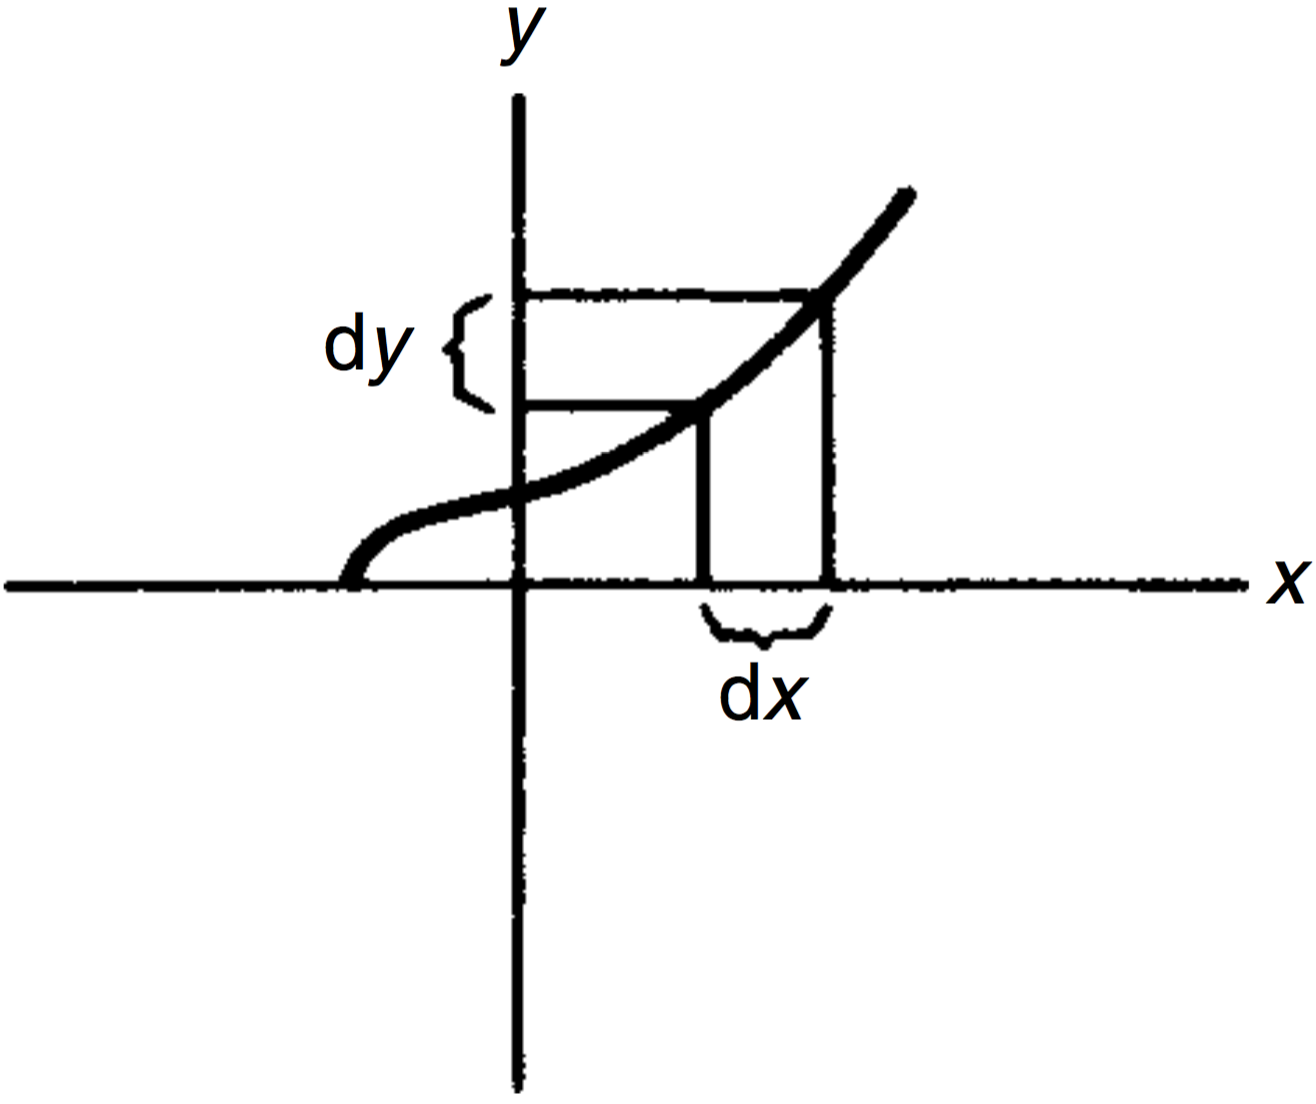
\includegraphics[width=0.4\textwidth]{graphics/gi/mc-10}
	\caption{$X$在$dx$区间的所有值被映射到$Y$在$dy$区间内}
	\label{f:pdf-map}
\end{figure}




\section{马尔可夫链蒙特卡洛方法}
到目前为止,前面讲述的对分布采样的方法称为直接采样法,在这种情况下概率分布通常是已知的,有些时候也能很容易地计算出归一化常数。然而直接采样方法在某些情况下会遇到困难甚至不适用,因此本章介绍另一种(也是非常重要的一种)基于马尔可夫链的梅特罗波利斯算法。

直接采样算法的遇到的第一个困难是,当随机变量的维度变得越来越高时,其采样效率变得越来越低,因此不适合于对高维分布进行采样。考虑随机向量: $X\sim f(x_1,x_2,\cdots,x_s )$,其中$s$为随机向量$X$的维度,每个分量的定义域为:$b_i-a_i$,则直接采样方法中取舍采样的效率为:

\begin{equation}
	\eta= \cfrac{1}{L}\prod^{s}_{i=1}(b_i-a_i)
\end{equation}

\noindent 其中,$L=\max{f(x_1,x_2,\cdots,x_s)}$,如果$L$值很大,或者维数$s$很高,则分母值很大,取舍算法的接受概率很低,拒绝率很高,因此采样效率非常低。直观上看,这是由于维数越高,用于包围目标概率分布的建议概率分布与目标概率分布之间存在更多的间隙空间,这些间隙空间即是被拒绝的采样点。

直接采样方法的另一个困难来自于概率分布为不完全已知概率分布,此时直接采样方法完全不适应。不完全已知概率分布是指,虽然概率分布的形式已知,但是其中包含部分项或本身就是很难进行数值计算的,例如为很难进行积分计算的高维积分,因此相当于是未知的。

一个直接的例子是渲染中每一帧图像的分布函数,我们可以将一张图像看成是某个值的概率分布,由于图像的每个像素的值是由RGB三个颜色值组成,因此这个值可以是这三个分量某种形式的函数,或者说我们可以以一个图像的亮度作为这个分布函数的值。在这个分布中,每一个像素位置的值是光线通过无数表面反射/折射传播的结果,因此每一个值本身就是一个高维积分计算,我们将在下一章看到渲染方程的路径形式,每一条路径都是一个高维积分。

本节要讨论的梅特罗波利斯算法是一种能够从任意概率分布$p(x)$中进行采样的方法,它提供一种机制使我们可以通过计算一个正比于目标分布函数$p(x)$的分布函数$f(x)$的值来获取采样值。由于$f(x)$只需要正比于目标分布,而不需要精确计算目标分布的归一化常数,因此梅特罗波利斯算法可以用于从任意分布采样。





\subsection{马尔可夫链}
梅特罗波利斯算法可以看做是取舍算法的一种推广,取舍算法每一步从建议分布产生一个全局的随机数,并与目标概率分布进行比较,以此来决定对新随机数的接受与拒绝,然而取舍算法的建议概率分布和目标概率分布之间的间隙随着随机变量维数的增加而增加,因此其效率极低。

而梅特罗波利斯算法以马尔可夫链为基础,整个取样的过程产生一条马尔可夫链,它将目标概率分布当做一个稳态的系统,每个新产生的随机数根据该系统的动态平衡关系进行取舍,所以最终整条马尔可夫链上的随机数序列就是服从目标概率分布的,并且梅特罗波利斯算法只需要能够计算目标概率分布每个定义域处的值,而不需要计算其归一化常数\footnote{注意:计算$p(x)$的每个值和计算$p(x)$的归一化常数是不一样的,后者实际上是积分${\rm \int} p(x){\rm d}x$的计算,这个积分计算可能非常困难。}。

所以为了理解梅特罗波利斯算法,我们需要首先了解马尔可夫链(Markov chain)\mathindex{马尔可夫链}{Markov chain}的概念及其属性,这是推导和理解梅特罗波利斯算法的重要基础。基于马尔可夫链的蒙特卡洛方法称为马尔可夫蒙特卡洛方法(Markov chain Monte Carlo, MCMC)\mathindex{马尔可夫蒙特卡洛方法}{Markov chain Monte Carlo},而梅特罗波利斯算法是最重要的一种马尔可夫蒙特卡洛方法。

设一个系统状态序列为$x_0,x_1,x_2,\cdots$,每个状态可以以一定的概率转移到另一个状态,假设我们从其中任意一个起始状态开始行走,每个时刻由一个状态转移到另一个状态(也可以转移到自身),如果对任何时刻$n$,系统状态的转移条件概率为:

\begin{equation}
	P(X_{n+1}=x|X_0=x_0,X_1=x_1,\cdots,X_n=x_n)=P(X_{n+1}=x|X_n=x_n)
\end{equation}

\noindent 则此转移过程形成的状态序列$X_0,X_1,\cdots,X_{n+1}$称为马尔可夫链\footnote{注意这里$X_n$表示$n$时刻产生的一个随机数,而$x_n$表示$n$时刻的一个系统状态值,其中两个相邻时刻的系统状态值可能是相同的。}。马尔可夫链的定义说明,其将来时刻$n+1$的状态,只依赖于当前时刻$n$的状态,与以前任何时刻的状态都无关。据此,系统状态序列$x_0,x_1,\cdots,x_n,x_{n+1}$发生的概率可分解为:

\begin{equation}
	P(x_0,x_1,\cdots,x_n,x_{n+1})=P(X_0=x_0)P(X_1=x_1|X_0=x_0)\cdots P(X_{n+1}=x_{n+1}|X_n=x_n)
\end{equation}

\noindent 式中,$P(X_0=x_0)$为初始状态的概率,通常是从初始状态$x_0$出发,所以$P(X_0=x_0)=1$;式中条件概率$P(X_{n+1}=x|X_n=y)$称为一步转移概率,简称为转移概率,表示在$n+1$时刻由$y$状态转移到$x$状态,转移概率通常与时刻$n$有关。若转移概率$P(X_{n+1}=x|X_n=y)$与时刻$n$无关,即$P(X_{n+1}=x_{n+1}|X_n=x_n)=P(X_n=x|X_{n-1}=y)$,则称马尔可夫链是均匀的,或者时齐的(time-homogeneous)\mathindex{时齐的}{time-homogeneous},通常我们研究的都是时齐的马尔可夫链,因此后面的表述我们将去掉时间$n$相关信息,$y$到$x$的状态条件转移概率直接表述为: $P(x|y)$。

马尔可夫链将一个系统的定义域当做一个状态空间,因此马尔可夫链又分为离散时间马尔可夫链(discrete-time Markov chain, DTMC)\mathindex{离散时间马尔可夫链}{discrete-time Markov chain}和连续时间马尔可夫链(continuous-time Markov chain, CTMC)\mathindex{连续时间马尔可夫链}{continuous-time Markov chain}。

马尔可夫链是在一个状态空间中从一个状态到另一个状态的不断转换的随机过程,这个过程中经过的每个状态值就是我们获得的服从这个状态空间概率分布的采样值。在一个平衡的系统状态中,每个状态到另一个状态的转移概率是固定的(我们可以将系统状态表述为一个状态图,如图\ref{f:mc-markov-chain}是一个具有两个状态的状态图),这些转移概率的结果就是使得状态空间的每个状态服从系统的分布,因此马尔可夫链是服从系统分布的一个随机采样序列。

初学者在理解马尔可夫链的时候往往比较吃力,这里尝试做一些解释,请读者细细体会。统计方法是关于用概率来解决确定性问题的方法,它的实际操作方式就是用大量的重复试验以获取足够的样本,而这些样本是满足目标概率分布的,所以能够用来解决确定性问题。具体地,以前面讲述的蒙特卡洛方法为例,当我们从一个概率分布$p(x)$采样产生一个随机数序列时,这个随机数序列里的值并不是唯一的,而是包含大量重复的值,每个随机数对应的概率越高,则其重现的次数越多,最终每个唯一随机数$x_i$在这个随机序列中出现的次数正比于它的概率$p_i$。

所以在马尔可夫链中也是一样,给定一个初始状态,马尔可夫链按照各个状态的转移概率在系统状态中随机行走,由于这些转移概率是按照系统状态的概率决定的,因此马尔可夫链就是一条状态链,这里马尔可夫链里出现的每个状态就是一个随机值,那些具有较高概率的系统状态,则其在马尔可夫链中出现的次数越多。因此,马尔可夫链本质上和前面讲述的其他采样方法是一样的,其目的都是产生服从目标概率分布的采样,但是操作方法不一样。

\begin{figure}
	\sidecaption
	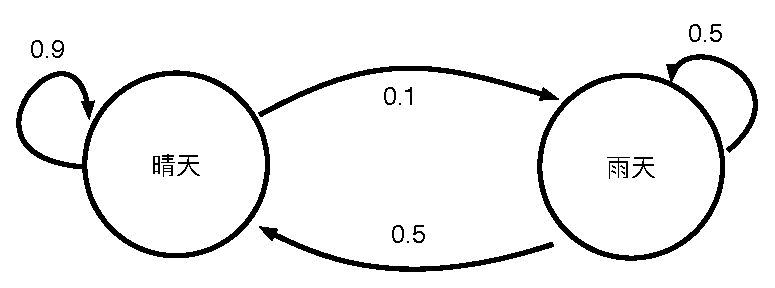
\includegraphics[width=0.6\textwidth]{figures/mc/markov-chain-example}
	\caption{一个具有两个转换状态的马尔可夫链(图片来自Wikipedia)}
	\label{f:mc-markov-chain}
\end{figure}

在一个给定平衡状态概率分布的系统中,如图\ref{f:mc-markov-chain}就是一个包含两个状态的系统,每个状态到其他状态的转移概率是固定的\footnote{实际上对于一个有限状态空间,整个系统状态的转移可以表述为一个转移矩阵,每个状态的矢量只需要乘以这个矩阵就能按照相关的概率进行转移,这里的例子参见:\url{https://en.wikipedia.org/wiki/Examples_of_Markov_chains};在本书后面的辐射度(radiosity)方法里,其思路就是将整个场景分成多个有限的面积块,然后由几何关系计算出每个面积块到其他面积块的转移比例,即是概率,然后给定任意一个光源,经过一定时间的反射,就能得到一个稳定的光照分布。},因此给定任意一个初始状态,例如晴天为$100\%$,雨天$0\%$,则等到一定时间$t$后系统处于平衡状态时,期间产生的马尔可夫链中晴天和雨天的分布一定服从平衡状态下的概率分布,即:约$83.3\%$的时间为晴天,剩下为雨天。

所以,利用马尔可夫链对目标概率分布进行采样的过程,实际上就是设一个状态系统服从目标概率分布,然后给定一个任意初始值,经历一定时间等系统趋于平衡之后,产生的马尔可夫链就是服从目标概率分布的,因此可作为服从该目标概率分布的采样值。由此也可以看出马尔可夫蒙特卡洛方法的一个问题,那就是开始一段趋近稳定状态的过程存在很大的方差,实践中往往需要通过某种方法省略掉这部分采样值。

而在马尔可夫蒙特卡洛方法中,梅特罗波利斯算法主要就是以一种简单的方式从已知概率分布中产生每个状态下正确的转移概率,要理解梅特罗波利斯算法的推导过程,我们还需要了解马尔可夫链的一些属性。




\subsubsection{马尔可夫链属性}
马尔可夫链有许多属性,为了简化概念,这里只讨论跟后面推导梅特罗波利斯算法相关的属性。


\paragraph{不可约性}
如果一个系统从状态$i$开始,存在非零的概率经过$n\geq 1$步之后可以达到状态$j$,则称$i$可达到(accessible)$j$,记为$i\rightarrow j$,表述为:

\begin{equation}
	P(X_{n_{ij}}=j|X_0=i)=p^{(n_{ij})}_{ij}>0
\end{equation}

如果$i\rightarrow j$和$j\rightarrow i$同时存在($n_{ij}$与$n_{ji}$可能不相等),则称$i$与$j$是联通的(communicating)。一个联通集合(communicating class)是指存在一个最大状态集合$C$,使得其中的每对状态相互都是联通的。

如果一个状态空间就是一个单一的联通集合,则称该状态空间内的马尔可夫链是不可约的(irreducible)\mathindex{不可约的}{irreducible},也就是说,在该状态空间中,可以由任何一个状态$i$出发,经过$n_{ij}$步之后,达到另外一个任意状态$j$。




\paragraph{非周期性}
假设从一个状态$i$出发,经过一定的步数$n_{ii}$后回到状态$i$自身,如果$n_{ii}$是$k$的倍数,则称状态$i$具有周期(period)$k$,称为周期态,一个状态的周期表述为:

\begin{equation}
	k=gcd\{n>0:P(X_n=i)|X_0=i)>0\}
\end{equation}

这里$gcd$表示取最大公约数\footnote{注意:即使状态$i$拥有最大公约数$k$,但并不意味着从$i$出发经过$k$步之后一定可以回到状态$i$,例如可能回到原状态的步数为$\{6,8,10,12,\cdots\}$,这里$k$为2,但是2并没有出现在返回步数列表中。}(greatest common divisor),如果$k=1$,则称该状态是非周期态(aperiodic state)\mathindex{非周期的态}{aperiodic state},它意味着回到状态自身的步数可以是任意的;如果至少有一个状态是非周期态,则称为非周期的马尔可夫链;若状态$i$的周期数$k>1$,则称其为周期态。



\paragraph{回返性}
假设从一个状态$i$出发,经过一定步数$n$之后回到状态$i$的概率记为:

\begin{equation}
	p^{(n)}_{ii}=P(T_i=n)
\end{equation}

\noindent 概率$p^{(n)}_{ii}$又称为首达概率,如果平均返回时间$T_i<\infty$,则称状态$i$为正回返(positive recurrent)状态,如果$T_i=\infty$,则称其为零回返状态,或者暂态(transient)。有限马尔可夫链的回返状态必为正回返状态。




\paragraph{遍历性}
如果状态$i$是正回返,不可约和非周期状态,则称状态$i$是各态遍历(ergodic)状态,或遍历态。换句话说,如果一个状态具有周期为1,并且能够在有限的平均步数内回返,则为遍历态。如果一个不可约的马尔可夫链中所有的状态都是遍历的,则该马尔可夫链是遍历的。

更一般地,如果一个马尔可夫链是遍历的,则始终存在一个步数$n$,使得从任意其他非$i$状态经过$n$步之后可以达到$i$状态。也就是说,马尔可夫链达到$i$状态的概率与初始状态无关,其实遍历性就是初始状态独立性。遍历性是马尔可夫链收敛到平稳分布的定量条件。




\paragraph{平稳分布}
设马尔可夫链在一个状态空间中从某个初始状态出发经历一定的时间后,各个状态$j$的离散分布概率为$\pi_{j}$,如果对任意状态$j$存在概率密度函数$\pi_j>0$,并使得:

\begin{equation}
	\sum^{n}_{i=1}\pi_i p_{ij}=\pi_j
\end{equation}

\noindent 即从所有其他状态转移到$j$状态的转移概率之和为状态$j$的概率分布,记为:

\begin{equation}
	\mathbf{\pi} \mathbf{P}=\mathbf{\pi}
\end{equation}

\noindent 则称马尔可夫链达到总体平衡,这里$\mathbf{P}$是一个转移矩阵,$\mathbf{\pi}$为所有状态的概率构成的矢量。一个正回返和非周期的马尔可夫链,当且仅当它是一个遍历链时,经历足够多的状态转移步数,这个马尔可夫链具有一个不变的概率分布$\pi_j>0$,这时无论初始分布如何,最终都会趋向于平稳概率分布$\pi_j$,于是有:

\begin{equation}
	\lim_{m\rightarrow \infty}p^{n}_{ij}=\pi_j
\end{equation}

这个唯一的近似不变的概率分布就是平稳分布(stationary distribution)\mathindex{平稳分布}{stationary distribution},它是一个极限分布。这就表明,最终状态不再发生变化,系统达到平稳状态。马尔可夫链具有平稳分布,是马尔可夫链的一个重要特征,在马尔可夫链蒙特卡洛方法中具有重要意义。

我们可以以前面的天气预报的状态分布为例来分析马尔可夫链从任意一个状态出发,经历一定时间后逐渐趋近于平稳分布的过程。如图\ref{f:mc-markov-chain}所示,这里状态空间的转移矩阵为:

\begin{equation}
	\mathbf{P}=\begin{bmatrix}
		0.9 & 0.1\\0.5 & 0.5
	\end{bmatrix}
\end{equation}

\noindent 设初始状态为晴天概率为$100\%$,雨天为$0\%$,用一个矢量表述为:

\begin{equation}
	\mathbf{x}^{(0)}=\begin{bmatrix}
		1.0&0.0
	\end{bmatrix}
\end{equation}

\noindent 则经过一次随机行走之后状态概率分布为:

\begin{equation}
	\mathbf{x}^{(1)}=\mathbf{x}^{(0)}\mathbf{P}=\begin{bmatrix}
		1.0&0.0 
	\end{bmatrix}\begin{bmatrix}
		0.9&0.1\\0.5&0.5
	\end{bmatrix}=\begin{bmatrix}
		0.9&0.1
	\end{bmatrix}
\end{equation}

\noindent 即依照这样的概率分布,第二天为晴天的概率为$90\%$,为雨天的概率相应为$10\%$,以此类推我们可以得到第$n$天的状态概率分布,如果$n$足够大,使系统趋近于稳定分布,则最终的天气预报的概率为:

\begin{equation}
	\begin{bmatrix}
		q_1&q_2
	\end{bmatrix}=\begin{bmatrix}
		0.833&0.167
	\end{bmatrix}
\end{equation}





\paragraph{细致平衡}
在一个状态空间中,如果存在概率分布$\pi$,使得:

\begin{equation}
	\pi_i p_{ij}=\pi_j p_{ji}
\end{equation}

\noindent 该条件称为细致平衡(detailed balance)\mathindex{细致平衡}{detailed balance},又称为局部平衡(local balance)。细致平衡是微观平衡,比上述的平稳分布(宏观平衡)具有更多的约束条件。

由细致平衡可以得到平稳分布,反之则不成立,平稳分布并不能保证细致平衡。满足细致平衡条件的马尔可夫链是可逆的\footnote{细致平衡本就是源于在一个平衡的动力学系统中,每个基础过程与其逆过程保持平衡。},称为可逆链,因此细致平衡与可逆性是等价的,可逆性保证了平稳分布。






\subsection{梅特罗波利斯算法}
有了平稳分布的条件,对于使用马尔可夫链的蒙特卡洛方法的思路则比较容易理解:它首先把目标概率分布的作用域看做一个状态空间,然后从任意一个状态出发随机行走以建立马尔可夫链,这个随机行走过程中的每一步遵循状态空间的转移概率分布,则经过一定时间之后,马尔可夫链中的状态概率分布会趋向于目标概率分布。在这个过程中,最重要的是怎样根据已知的目标概率求出转移概率分布,梅特罗波利斯算法(Metropolis algorithm)\mathindex{梅特罗波利斯算法}{Metropolis algorithm}的核心就是使用了一种简单求解转移概率的方法。

为了更好地理解梅特罗波利斯算法及其最关键的概念,我们有必要区分一下统计学中利用马尔可夫链解决积分问题的两种不同的思路:第一种是已知目标概率分布$p_i$,使用蒙特卡洛方法对这个目标概率分布进行采样,然后计算积分,此种方法的关键是要根据已知目标概率求出状态转移概率$p_{ij}$,这样使得马尔可夫链能够逼近目标分布,这即是本节讨论的梅特罗波利斯算法;第二种是已知转移概率分布,然后给定任意一个初始概率分布,则马尔可夫链会根据转移概率逐渐趋向于稳定分布,这种思路在计算机图形学中被用于本书后面第\ref{chp:rad}章会讨论的辐射度方法(radiosity)\mathindex{辐射度方法}{radiosity}中;当然后者是一种迭代法(而不是蒙特卡洛方法),但是它与马尔可夫链性质的运用其实有很深的联系,在学习辐射度理论的时候可以细细体会这种联系。

梅特罗波利斯算法通过逐渐产生一序列的随机数的方式工作,这个随机数序列是以迭代的方式产生的,在这个迭代的过程中,下一个随机数的产生仅依赖于上一个随机数(因此整个随机数序列是一个马尔可夫链),随着产生越来越多的随机数,这个随机数序列会逐渐逼近于目标概率分布。

特别地,在每一次迭代中,该算法基于当前随机数产生一个新的候选随机数,然后这个候选随机数根据一定的概率被接受(这种情况下新的候选随机数会被用于下一个迭代中)或拒绝(这种情况下新的候选随机数被丢弃,当前随机数继续被用在下一个迭代中),这个接受概率被适当选取以使其能够近似目标概率的分布。

设$f(x)$为一个正比于目标概率分布$p(x)$的近似分布,梅特罗波利斯算法的基本步骤如下:

\begin{enumerate}
	\item 初始化阶段:选取一个任意点$x_0$作为起始采样点,并选择一个任意概率密度函数$g(x|y)$用来根据当前采样随机数$y$产生下一个候选随机数$x$,在梅特罗波利斯算法中,$g$必须是对称的,即满足$g(x|y)=g(y|x)$。一个常用的选择是高斯分布(Gaussian distribution)\mathindex{高斯分布}{Gaussian distribution},也即正态分布(normal distribution)\mathindex{正态分布}{normal distribution},这种情况下,靠近$y$的点会被以更高的概率成为候选采样点。$g$被称为建议密度函数(proposal density function)\mathindex{建议密度函数}{proposal density function}或跳跃分布(jumping distribution)\mathindex{跳跃分布}{jumping distribution}。
	\item 迭代阶段,对于每一次迭代$n$:
	\begin{itemize}
		\item 首先从建议密度函数$g(x^{'}|x_n)$产生一个候选采样点$x^{'}$。
		\item 计算接受率$\alpha= \cfrac{f(x^{'})}{f(x_n)}$,这个接受率用于决定新的候选采样点被接受或拒绝。因为$f(x)$正比于目标概率密度函数$p(x)$,所以$\alpha= \cfrac{f(x^{'})}{f(x_n)}= \cfrac{p(x^{'})}{p(x_n)}$。
		\item 如果$\alpha\geq 1$,新的候选点直接被接受:$x_{n+1}=x^{'}$;否则,按照概率$\alpha$来接受新的候选点,如果新的候选点被拒绝,则设置:$x_{n+1}=x_n$。
	\end{itemize}
\end{enumerate}

梅特罗波利斯算法的过程是通过在采样空间随机行走实现,在随机行走的每一步,新的随机采样点可能被接受,也可能被拒绝,这完全由接受率$\alpha$来决定。接受率$\alpha$表述的是根据目标概率分布$p(x)$,新产生的候选随机数相对于当前随机数有多大的概率被接受,例如如果$\alpha\geq 1$,说明新的候选采样点$x^{'}$在$p(x)$中处于更高概率区域,即是它比$x_n$具有更高的概率,因此新的候选点总是被接受;如果$\alpha<1$,则说明新的候选点在$p(x)$中处于较低概率区域,此时它可能会被接受,可能会被拒绝,$\alpha$越小,新的候选点拥有更小的几率被接受。因此,通过这样的机制,马尔可夫链中的随机数倾向于停留在目标概率分布$p(x)$的高概率区域,而只有偶尔很少的机会会访问低概率区域。直观上看,这就是梅特罗波利斯算法能够工作的原因,也使它最终返回的采样点是符合目标概率分布的。





\subsubsection{收敛性证明}
梅特罗波利斯算法的目标是根据目标概率分布$p(x)$产生一个状态序列,为了达到这个目的,它使用一个马尔可夫过程来渐渐地逼近一个唯一的稳定分布$\pi(x)$,使得$\pi(x)=p(x)$。那么怎样证明该算法是收敛于$p(x)$的呢?

马尔可夫链蒙特卡洛方法的各种算法的收敛性是基于马尔可夫链的收敛性理论。一个马尔可夫过程由其转移概率$P(x^{'}|x)$唯一决定,要使该马尔可夫过程存在一个唯一的稳定分布$\pi(x)$,必须满足以下两个条件:

\begin{enumerate}
	\item 存在稳定分布。
	\item 稳定分布是唯一的。
\end{enumerate}

要使马尔可夫链存在稳定分布,由前面的内容可知,一个充分不必要条件是满足细致平衡(detailed balance)\myindex{细致平衡}{detailed balance}条件,细致平衡条件要求每个转移过程是可逆的,对于每一对状态$x$和$x^{'}$,处于状态$x$并转移到状态$x^{'}$的概率必须等于处于状态$x^{'}$并转移到状态$x$的概率,即:$\pi(x)P(x^{'}|x)=\pi(x^{'})P(x|x^{'})$。

稳定分布的唯一性可以由遍历性(ergodicity)\myindex{遍历性}{ergodicity}来保证,通过前面的马尔可夫链属性可知,马尔可夫链的遍历性必须要求非周期性和正回返性。非周期性其实暗指每个状态不是只能从某些特定路径返回,而是可以沿任意路径返回,其意义就是每个状态可以与任意状态联通;而正回返性保证这种联通的概率小于$\infty$。由不可约性可知,如果状态空间内所有状态都是联通的,从每个状态出发经过一定步数之后都可以达到另一个状态,则马尔可夫链就是与初始状态无关的,所以遍历性保证了稳定分布的唯一性。

梅特罗波利斯算法就是通过设计一个满足上述两个条件的马尔可夫链,以使稳定分布$\pi$逼近$p(x)$。该算法的推导首先从满足细致平衡条件开始:

\begin{equation}
	P(x^{'}|x)p(x)=P(x|x^{'})p(x^{'})
\end{equation}

\noindent 上式可以改写为:

\begin{equation}
	 \cfrac{P(x^{'}|x)}{P(x|x^{'})}= \cfrac{p(x^{'})}{p(x)}
\end{equation}

梅特罗波利斯算法将转移概率的计算分成两步:建议概率$g(x^{'}|x)$和接受率$\alpha(x^{'}|x)$,并使得:

\begin{equation}
	P(x^{'}|x)=g(x^{'}|x)\alpha(x^{'}|x)
\end{equation}

\noindent 将上式代入前面的细致平衡关系,得到:

\begin{equation}
	 \cfrac{\alpha(x^{'}|x)}{\alpha(x|x^{'})}= \cfrac{p(x^{'})}{p(x)} \cfrac{g(x|x^{'})}{g(x^{'}|x)}
\end{equation}

\noindent 接下来就是怎么选择接受概率$\alpha$以满足上面的条件,由前面的梅特罗波利斯算法可知其选择为:

\begin{equation}
	\alpha(x^{'}|x)=\min \bigg( 1, \cfrac{p(x^{'})}{p(x)} \cfrac{g(x|x^{'})}{g(x^{'}|x)}\bigg)=\min\bigg(1, \cfrac{p(x^{'})}{p(x)}\bigg)
\end{equation}

上式后半部分的等式成立是因为梅特罗波利斯算法中建议概率$g$是对称的,从此也可以看出,梅特罗波利斯算法中中的建议概率$g$是可以任意选择的,因为它并不会参与到最终转移概率的计算上。梅特罗波利斯算法中的转移概率是满足细致平衡条件\footnote{对于好奇的读者可以由以下证明过程证明其满足细致平衡条件:
\begin{equation}
	\begin{aligned}
		p(x)P(y|x)&=p(x)g(y|x)\alpha(y|x)=p(x)g(y|x)\min(1,p(y)/p(x))\\
		&=\min(p(x)g(y|x),g(y|x)p(y))=p(y)g(x|y)\min(p(x)/p(y),1)\\
		&=p(y)g(x|y)\alpha(x|y)=p(y)P(x|y)
	\end{aligned}
\end{equation}
}的,而细致平衡条件可以保证稳定分布,也就是总体平衡,因此梅特罗波利斯算法是收敛的。





\subsubsection{梅特罗波利斯算法的不足}
尽管梅特罗波利斯算法中是收敛的,但是马尔可夫链蒙特卡洛方法的各种算法收敛性证明只能证明其样本值遵从已知概率分布,但不能证明样本值是独立无关的,也没有给出收敛速度是多少。本节介绍梅特罗波利斯算法主要的两个方面的不足。

首先,尽管梅特罗波利斯算法的建议概率$g$可以是任意选取的,并且能够保证收敛性,但是它的选取却对效率和方差由一定的影响。直观上,为了使马尔可夫链收敛的速度更快,以及更快地遍历整个状态空间,我们趋向于选取步幅更大的建议概率。但是对于用于高频率分布的目标分布函数,过大的建议步幅在高频部分将导致$p(x^{'})\gg p(x)$,因此使得接受率$\alpha$非常低,其结果就是大量的随机数停留在尖锐的区域,导致方差增大,并且收敛速度变慢(随机数被卡在高频部分很长时间),如图\ref{f:mc-met-1}所示;相反,过小的建议步幅则会直接导致更慢的收敛速度,所以合适地选取建议概率函数非常重要,我们将在后面第\ref{chp:mlt}章学习MLT算法的时候更具体地讨论一些建议概率函数选择的策略。

\begin{figure}
	\sidecaption
	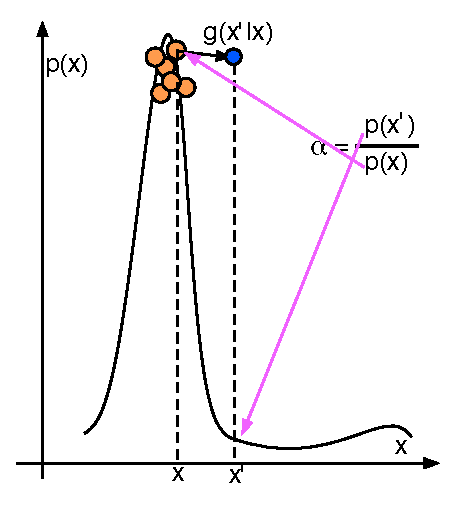
\includegraphics[width=0.4\textwidth]{figures/mc/metropolis-1}
	\caption{如果分布函数的某些区域比较尖锐,或者由于建议概率产生的候选随机数的步幅过大,则会导致大部分候选随机数由于接受率$\alpha$太低而被拒绝,因此在尖锐的部分聚集大量相同的随机数,导致方差增大}
	\label{f:mc-met-1}
\end{figure}

其次,虽然梅特罗波利斯算法最终会收敛于目标概率分布,但是在这个收敛的过程中,一些初始的随机数序列则可能完全不是服从目标概率分布的,这部分随机数通常需要从马尔可夫链中去除掉,然而并没有一些好的算法用于预测这个收敛的长度需要多少初始随机数。

尽管如此,梅特罗波利斯算法能够轻松应对高维概率分布的采样是其他方法不可比拟的,有时候几乎梅特罗波利斯算法是唯一的选择。在本章中我们仅介绍梅特罗波利斯算法的一些基本概念,在第\ref{chp:mlt}章还会有更多更具体的内容来讨论梅特罗波利斯算法的一些取舍以及更多的实现细节。





\section{方差缩减}\label{sec:Variance-Reduction}
通过前面的内容,我们已经熟悉了使用蒙特卡洛方法求积分的基本方法,这里再总结一遍,它基本上可以分为三个步骤:首先,使用前面讲述的一些采样方法(如逆向变换算法)从一个目标概率分布中采样产生一系列随机数$x_i$;接着,将每个随机数代入式$ \cfrac{f(x_i)}{p(x_i)}$中求得每个样本的统计值;最后,求出这些统计值的平均值用来近似(估计)函数$f(x)$的积分。

由于蒙特卡洛方法是一个统计过程,因此方差始终存在,设计更有效的估计是蒙特卡洛方法研究中的主要领域,从蒙特卡洛方法诞生至今已出现非常多的方差缩减(variance reduction)\mathindex{方差缩减}{variance reduction}的方法,但是由于蒙特卡洛方法在图形学中的运用往往都是要求计算不要太复杂,所以本节仅介绍少数几种计算机图形学中常用的方差缩减方法。





\subsection{重要性采样}
重要性采样(importance sampling)\mathindex{重要性采样}{importance sampling}是蒙特卡洛方法中最基础也是非常重要和有效的方差缩减方法,它通过选择对一个与目标概率分布具有相似形状的分布函数进行采样来减少方差。直观上看,重要性采样试图在被积函数中贡献更高的区域放置更多的采样点,以体现这部分区域的重要性。

给定一个概率分布$p(x)$,以及从该分布采样得到的$N$个随机数$x_i$,根据蒙特卡洛方法,被积函数$f(x)$的积分$I$可以通过以下式来进行估计:

\begin{equation}
	I_N= \cfrac{1}{N}\sum_{i=1}^{N} \cfrac{f(x_i)}{p(x_i)}
\end{equation}

一个完美估计(perfect estimator)的方差应该为0,由此,相对理想的采样概率密度函数$p(x)$可以从下式推导出:

\begin{equation}
	0=\sigma^2= \cfrac{1}{N}{\rm \int}( \cfrac{f(x)}{p(x)}-I)^2p(x){\rm d}x
\end{equation}

\noindent 因为$p(x)$是非零的,所以:

\begin{equation}
	p(x)= \cfrac{|f(x)|}{I}
\end{equation}

如果我们使用这样的概率密度函数进行采样,其方差会被完美地消除,然而,这个理想的$p(x)$要求我们首先计算出$I$的值,而这正是我们试图去求解的,因此找到这样理想的$p(x)$是完全不可能的。

不过,我们可以选择和被积函数$f(x)$具有相似形状的概率密度函数来减少方差,直观上理解,它使得每个样本值$ \cfrac{f(x_i)}{p(x_i)}$趋近于一个常数,也即是通过减少每个$ \cfrac{f(x_i)}{p(x_i)}$值的变化范围来减少方差,因为常数的方差为0。

\begin{figure}
	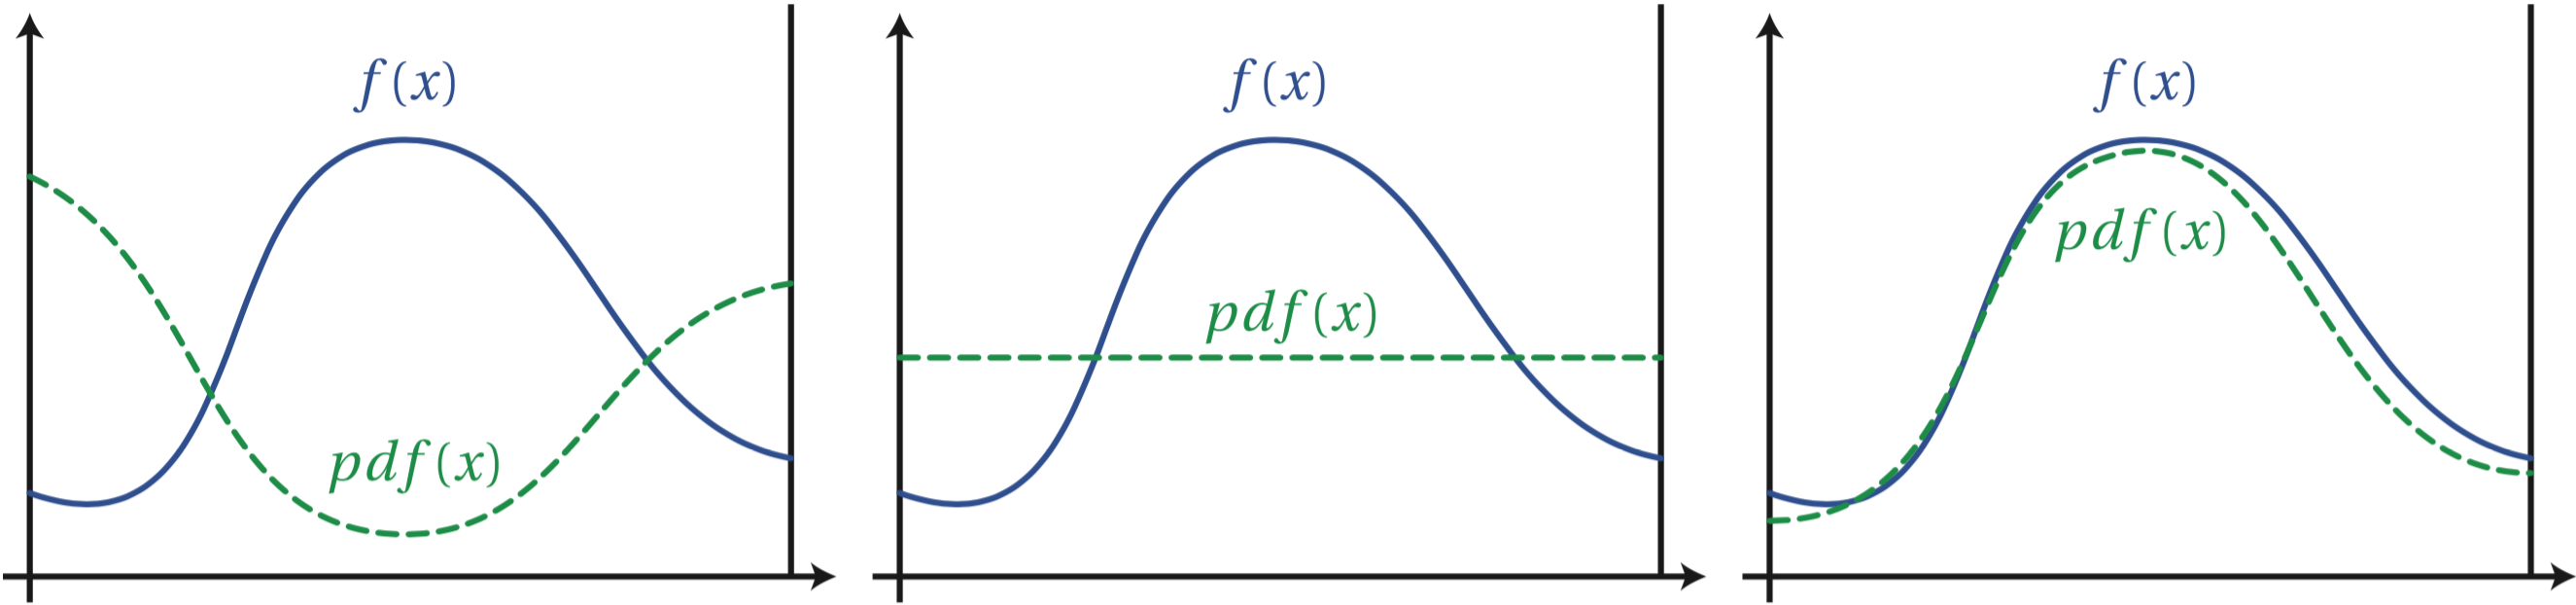
\includegraphics[width=\textwidth]{figures/mc/mc-11}
	\caption{重要性采样(右图)通过选择和被积函数具有相似形状的概率密度函数来进行采样,以减小统计方法导致的方差;此外,任意选择的分布(左图)可能比均匀分布(中图)具有更大的方差}
	\label{f:mc-importance-sampling}
\end{figure}

图\ref{f:mc-importance-sampling}展示了选择不同的概率密度函数$p(x)$对被积函数$f(x)$估计的差异,右边小图的重要性采样会比左图任意分布采样以及中间小图的均匀采样拥有更小的方差,此图也说明任意选择的采样(左边小图)可能比使用均匀分布(中间小图)的方差要大很多。所以从这里可以看出选择用于产生采样的概率密度函数的重要性,尽管蒙特卡洛方法本身没有限制对概率密度函数的选择,但是选择不好的概率密度函数会大大增加蒙特卡洛估计的方差。





\subsection{复合重要性采样}\label{sec:mc-mis}
在实际的情景中,计算机图形学中的被积函数通常是具有非常复杂,不正常的分布的,它们可能是不连续的,通常在少数区域拥有奇点(singularities)或者一些较大的值,所以很难找到一个简单的与其被积函数相似的分布用来进行重要性采样。

例如,考虑渲染中最普通的直接光源的计算,其公式如下:

\begin{equation}
	L_o({p},\mathbf{v})={\rm \int}_{\Omega}f_r(\mathbf{l},\mathbf{v})\otimes L_i({p},\mathbf{l})\cos\theta_i {\rm d}\omega_i
\end{equation}

我们可能选择$L_i$或$f_r$来进行重要性采样,但是这两者都会产生糟糕的结果,因为一个不好的分布比均匀分布的方差要更大。考虑一个接近镜面的BRDF的表面被一个面积光照射的例子,如图\ref{f:mc-mis}所示,这里面积光源的分布$L_i$被用来作为采样函数,因为BRDF是几乎镜面的,所以除了沿镜面反射光方向$\omega_i$,大部分光源上的采样对最终光照的贡献几乎为0,因此估计的方差会非常大;虽然这种情况下使用BRDF分布作为采样分布比较合适,但是对于被很小面积光源照射的漫反射或高光表面,使用BRDF作为采样分布仍然会导致很大的方差,此时我们应该尽可能地在光源上产生更多地采样点。

因此,我们通常需要使用更复杂的采样方式(而不是简单地从一个简单分布采样)以使估计具有更低的方差,这通常涉及根据被积函数的分布特征对其进行区域划分,然后在不同特征的区域上使用不同的分布函数进行采样,最后再将这些结果以某种方式进行混合。

\begin{figure}
	\begin{subfigure}[b]{0.328\textwidth}
		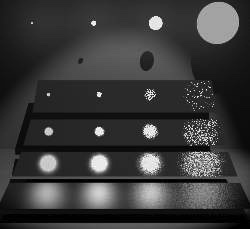
\includegraphics[width=1.0\textwidth]{figures/mc/mis-1}
		\caption{根据光源分布采样}
	\end{subfigure}
	\begin{subfigure}[b]{0.328\textwidth}
		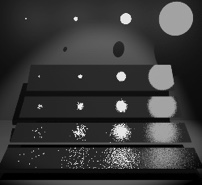
\includegraphics[width=1.0\textwidth]{figures/mc/mis-2}
		\caption{根据BRDF分布采样}
	\end{subfigure}
	\begin{subfigure}[b]{0.328\textwidth}
		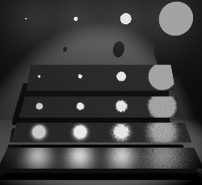
\includegraphics[width=1.0\textwidth]{figures/mc/mis-3}
		\caption{复合重要性采样}
	\end{subfigure}
	\caption{对于一个被面积光照射的高光表面的直接光进行采样,这里有4个圆形面积光源,它们分别拥有不同的辐射照度及颜色,在四个圆形光源上面是一个聚光灯光源,所有的光源具有相同的辐射能量;下面是4个拥有不同粗糙度的高光矩形塑料(图片来自\cite{a:OptimallyCombiningSamplingTechniquesforMonteCarloRendering})}
	\label{f:mc-mis}
\end{figure}

复合重要性采样(multiple importance sampling,MIS)\mathindex{复合重要性采样}{multiple importance sampling}就是这样一类采样方法,它非常简单而有效,它提供一个策略使得可以从多个不同的分布中采样,然后对这些不同的采样结果进行加权组合。根据原始论文\cite{a:OptimallyCombiningSamplingTechniquesforMonteCarloRendering},复合重要性采样可以简单地分为以下几步:

\begin{itemize}
	\item 首先,选择一系列的重要性分布$p_1,...,p_n$,使得对于被积函数$f$的每一个潜在值比较大的区域$\Omega_i$,在那个区域它能够被其中的一个单个重要性分布$p_i$近似(形状相似),如图\ref{f:mc-mis-example}所示。通常一个复杂的被积函数是多个不相关的简单分布的乘积的形式,所以这些重要性分布的最佳来源就是这些简单分布,使得$p_i$可以正比于每个简单分布。
	\item 然后,从每个分布$p_i$产生$n_i$个随机数$X_{i,1},\cdots,X_{i,n_i}$,这通常是根据某种策略基于$f$和$p_i$提前(在采样之前)计算而出。
	\item 最后,对每个分布的结果使用一个组合估计(combined estimator)进行加权组合以对积分进行估计。 
\end{itemize}

复合重要性采样中的组合估计表达式如下:

\begin{equation}\label{e:combined-estimator}
	I_N=\sum_{i=1}^{n} \cfrac{1}{n_i}\sum_{j=1}^{n_i}\omega_i(X_{x,j}) \cfrac{f(X_{i,j})}{p_i(X_{i,j})}
\end{equation}

上式说明复合重要性采样是多个重要性采样的一个加权组合,它将整个空间按一定的形式划分,然后对每个划分的区域使用不同的采样技术,所以$\sum^{n}_{i=1}$表示的就是这些不同采样技术的和;$\sum^{n_i}_{j=1}$表示一种特定的采样技术$p_i$的估计值,但是由于在每个$f(x){\rm d}x$区间内,每种技术只贡献其中一部分值,所以每种技术的估计结果被乘以一个系数$\omega_i(X_{i,j})$,$\omega_i(x)$可以在每个$x$处的值不一样,只要保证对于每个$x$位置处满足$\sum^{n}_{i=1}\omega_i(x)=1$就行,这样就能保证每个$x$处的值被正确估计。

\begin{figure}
	\sidecaption
	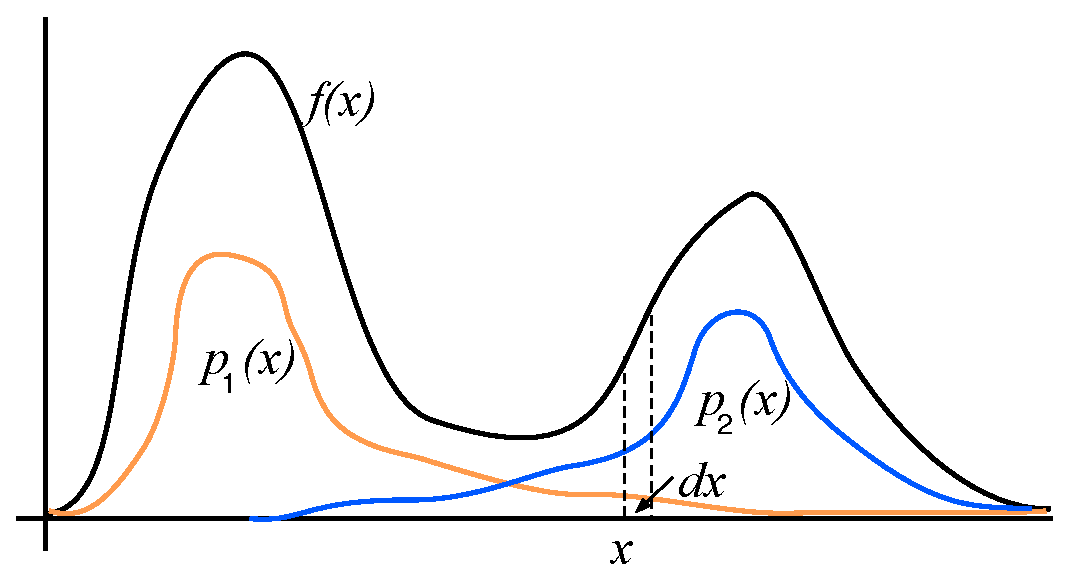
\includegraphics[width=0.55\textwidth]{figures/mc/mis}
	\caption{复合重要性采样对多个采样技术进行组合,即加权和,并可以根据每个区域内多个采样技术的贡献度来调整混合权重,使得联合估计结果能够充分发挥每个采样技术的优势}
	\label{f:mc-mis-example}
\end{figure}

我们可以再解释一下这个加权系数$\omega_i(x)$的由来及原理,假设现有两个采样技术$p_1(x)$和$p_2(x)$如图\ref{f:mc-mis-example}所示,两种采样技术单独的采样结果分别为$ \cfrac{1}{n_1}\sum \cfrac{f(x)}{p_1(x)}$和$ \cfrac{1}{n_2}\sum \cfrac{f(x)}{p_2(x)}$,它们都分别能够完全估计目标积分$I$,但是各自的方差都很大。所以我们使用将两种采样技术进行组合,所以每个采样的区域是两个采样技术的加权和,为了尽可能发挥每个采样技术的优势,我们往往尽可能保证在每个区域贡献更高的采样技术拥有更高的权重,这也正是后面平衡启发式的原理。

我们可以证明复合重要性采样的联合估计是无偏的:

\begin{equation}
	E[I_N]=\sum_{i=1}^{n} \cfrac{1}{n_i}n_i{\rm \int}_{\Omega} \cfrac{\omega_i(x)f(x)}{p_i(x)}p_i(x){\rm d}\mu (x)={\rm \int}_{\Omega}f(x){\rm d}\mu (x)
\end{equation}

基于以上联合估计,我们可以选择使用不同的权重系数$\omega_i(x)$来混合多个采样分布,以尽可能减少估计的方差。




\subsubsection{平衡启发式}\label{sec:mc-balance-heuristic}
考虑如下的权重系数函数:

\begin{equation}
	\hat{\omega}_i(x)= \cfrac{c_ip_i(x)}{\sum_j c_jp_j(x)}
\end{equation}

\noindent 这里$c_i$是每个采样分布$p_i$对应的采样数量的比例,$c_i= \cfrac{n_i}{N}$,所以$\sum_i c_i=1$,$c_i$是一个固定的数值,它在采样之前确定。这个权重系数函数$\hat{\omega}_i(x)$拥有一个属性,那就是采样值$ \cfrac{\hat{\omega}_i(x)f(x)}{n_ip_i(x)}$完全与$i$无关,因为每个$x$的采样值对于所有采样技术都是无关的,所以我们称这种策略为平衡启发式(balance heuristic)\mathindex{平衡启发式}{balance heuristic}。

代入$\hat{\omega}_i$到式\ref{e:combined-estimator},我们得到标准的蒙特卡洛估计:

\begin{equation}
	I_N= \cfrac{1}{N}\sum_{i=1}^{n}\sum_{j=1}^{n_i} \cfrac{f(X_{i,j})}{\overline{p}(X_{i,j})}
\end{equation} 

\noindent 这里:

\begin{equation}
	\overline{p}(x)=\sum_{i=1}^{n}c_ip_i(x)
\end{equation}

$\overline{p}(x)$又称为联合采样分布(combined sample distribution)\mathindex{联合采样分布}{combined sample distribution},对于总数$N$个采样,其中每个$n_i=c_i N$个独立的随机数$X_{i,j}$分别从分布$p_i$采样而得。

这就是平衡启发式的核心思想,也是一种很自然的组合多种采样技术的方式。我们使用一个单一的与$i$完全无关的分布$\overline{p}(x)$来表述这种组合方式。更进一步理解,$\overline{p}(x)$是一个由每个$X_{i,j}$组成的随机变量$X$的分布,每个随机数的概率为$1/N$。

除了平衡启发式,还存在一些其他的不同形式的混合系数函数,感兴趣的读者可以参考 \cite{a:Safeandeffectiveimportancesampling,a:AdaptiveMultipleImportanceSampling,a:ANADAPTIVEPOPULATIONIMPORTANCESAMPLER,a:EfficientMultipleImportanceSamplingEstimators}等。





\subsection{分层采样}
重要性采样技术在被积函数更重要的区域放置更多的随机数来更好地逼近原始分布,然而它并不能消除由于随机数导致的丛聚(clumping)\mathindex{丛聚}{clumping},由于概率密度函数产生的随机数仅仅指示的是一个期望值,而不是一个绝对的数量。这些丛聚现象会导致估计的方差增大,因为它可能导致其他某些区域可能被忽略了。

与重要性采样调整采样函数$p(x)$的思路不同,针对上述问题,另一类常见的方差缩减的技术基于小心地设置采样随机数在被积函数区域的放置,其目标是使它们能够捕捉到被积函数的各部分重要信息(不至于由于随机数的丛聚导致某些部分被忽略),这类方法的结果是随机数不再是完全随机的,这类方法通常用作重要性采样等技术的一种补充。本节我们讨论分层采样技术,而下一节讨论完全非随机的拟蒙特卡洛方法。

分层采样(stratified sampling)\mathindex{分层采样}{stratified sampling}将被积函数的定义域$\Omega$划分成多个彼此不相交的子定义域$\Omega_1,...,\Omega_n$,即满足:

\begin{equation}
	\bigcup_{i=1}^{n}\Omega_i=\Omega
\end{equation}

\noindent 每个子定义域$\Omega_i$称为一个阶层(stratum)\mathindex{阶层}{stratum},在每个阶层$\Omega_i$内,固定数量的$n_i$个随机数分别从采样分布$p_i$采样而得。在每个阶层内,其蒙特卡洛估计为:

\begin{equation}
	F_i= \cfrac{1}{n_i}\sum_{j=1}^{n_i} \cfrac{f(X_{i,j})}{p_i(X_{i,j})}
\end{equation} 

\noindent 这里,$X_{i,j}$是从采样分布$p_i$中采样产生的第$j$个随机数,因此整个被积函数的估计为:

\begin{equation}
	F=\sum_{i=1}^{n}v_iF_i
\end{equation}

\noindent 这里$v_i$表示每个阶层$i$ ($v_i\in(0,1]$)占整个定义域空间的体积的比例,该估计的方差为:

\begin{figure}
\sidecaption
	{\begin{subfigure}[b]{0.3\textwidth}
		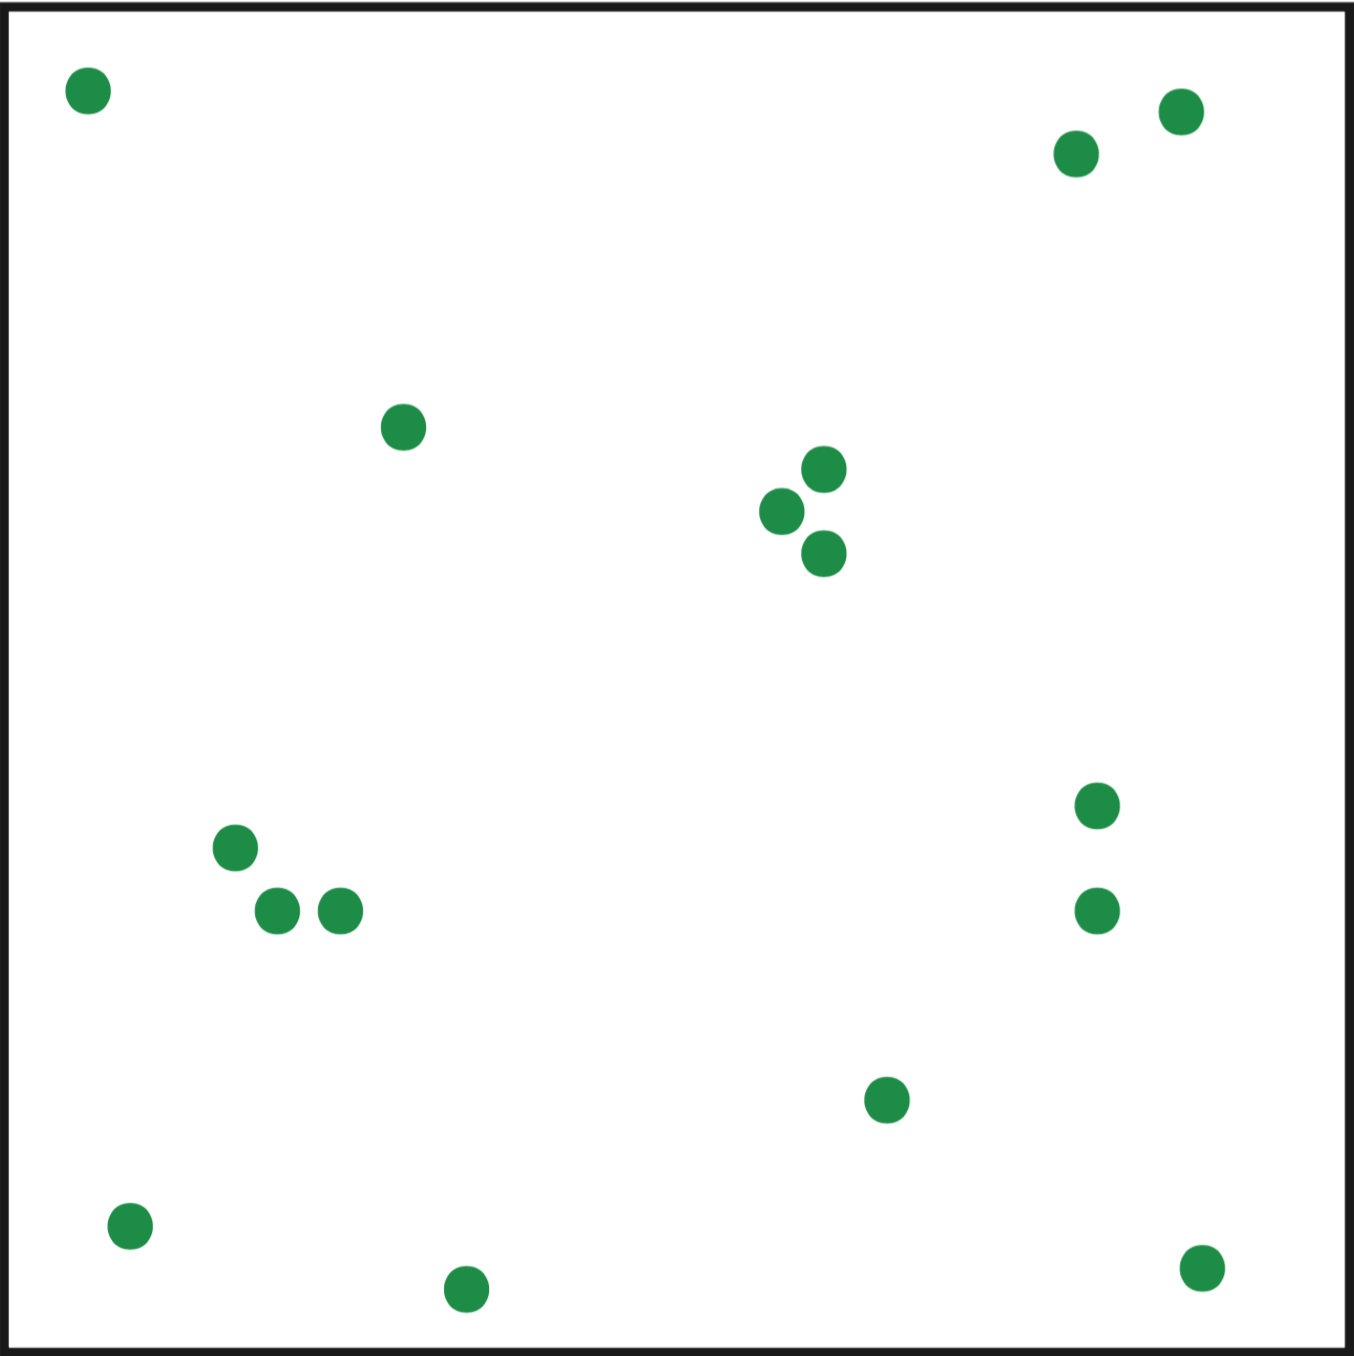
\includegraphics[width=1.\textwidth]{figures/mc/mc-12-1}
		\caption{随机采样}
	\end{subfigure}
	\begin{subfigure}[b]{0.3\textwidth}
		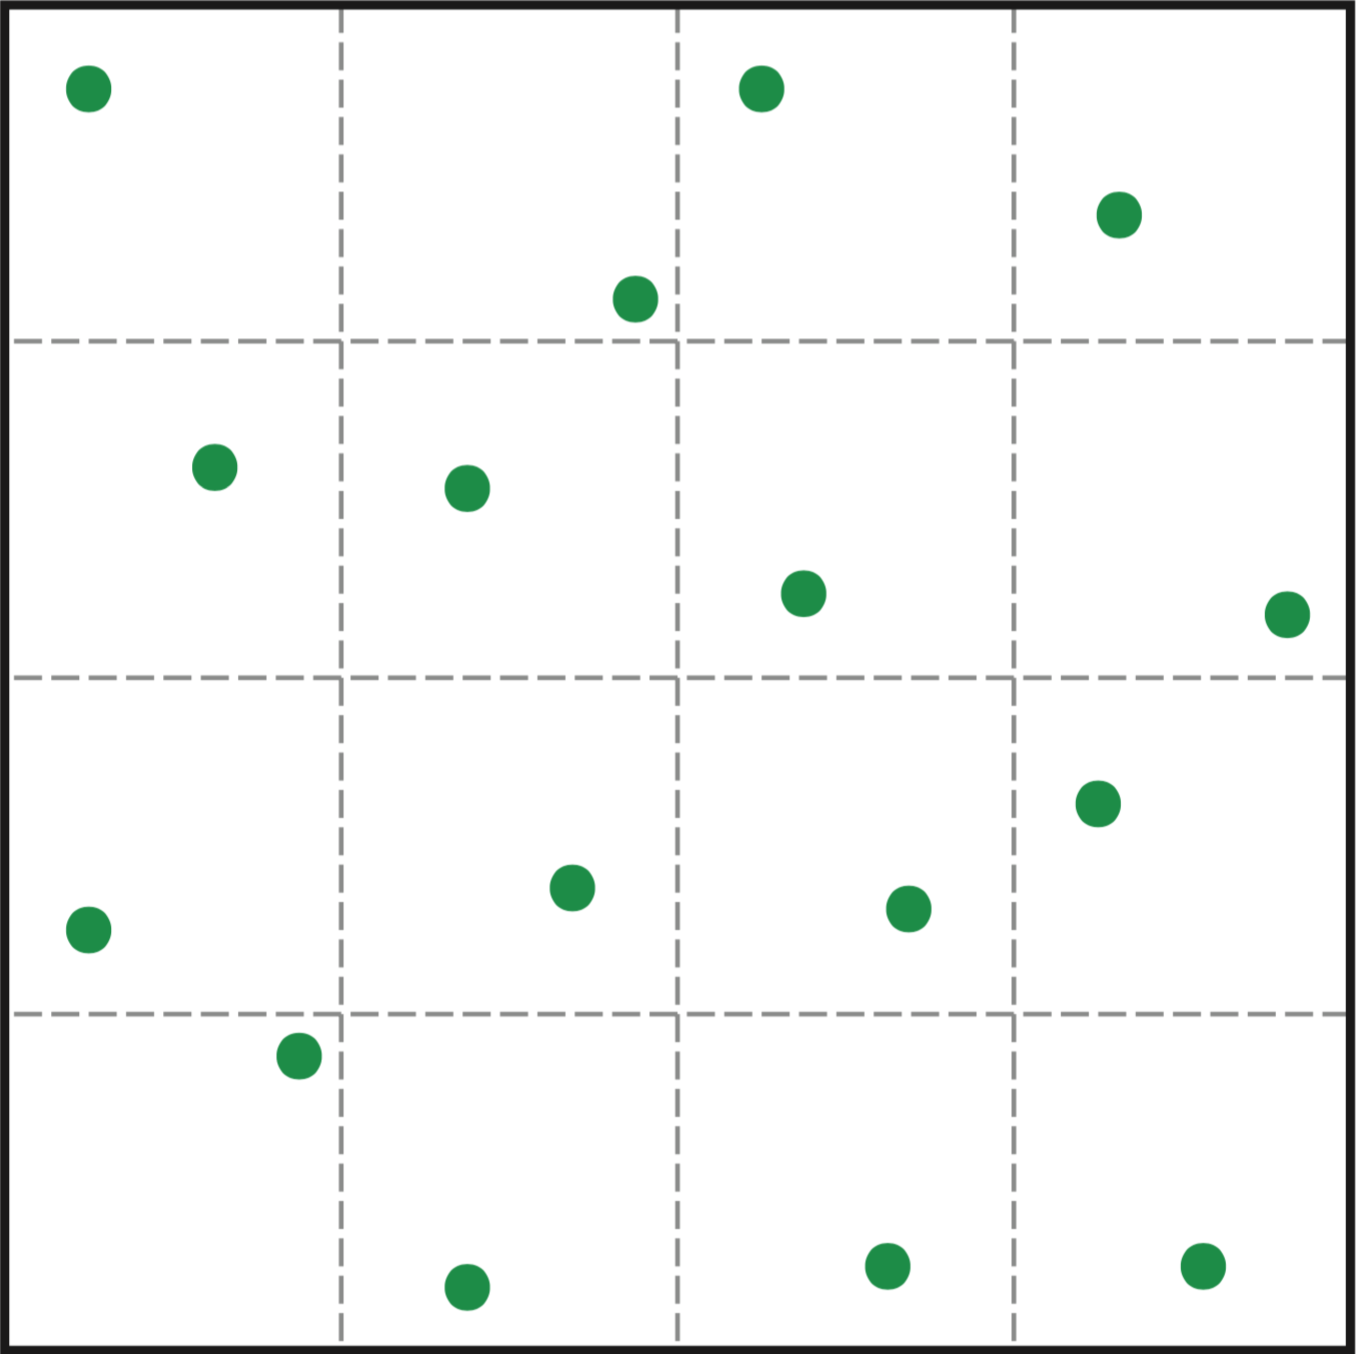
\includegraphics[width=1.\textwidth]{figures/mc/mc-12-2}
		\caption{分层采样}
	\end{subfigure}}
	\caption{16个随机采样值和分层采样的比较,完全随机的采样(a)可能会导致丛聚,丛聚可能使得被积函数其他区域采样不足从而增加估计的方差}
	\label{f:placement}
\end{figure}


\begin{equation}
	V[F]=\sum_{i=1}^{n} \cfrac{v_{i}^2 \sigma_{i}^2}{n_i}
\end{equation}

\noindent 这里$\sigma_{i}^2=V[f(X_{i,j})]$表示在阶层$\Omega_i$内的估计的方差。

为了与其他非分层采样方法进行比较,假设$n_i=v_iN$,$N$为估计全部使用的样本,上式可以简化为:

\begin{equation}
	V[F]= \cfrac{1}{N}\sum_{i=1}^{n}v_{i} \sigma_{i}^2
\end{equation}

另一方面,非分层采样估计的方差可以表示为(感兴趣的读者可以参见\cite{a:RobustMonteCarloMethodsforLightTransportSimulation}第51页的推导过程):

\begin{equation}
	V[F]= \cfrac{1}{N}\Bigg[ \sum_{i=1}^{n}v_{i} \sigma_{i}^2 +\sum_{i=1}^{n}v_i(\mu_i-I)^2   \Bigg]
\end{equation}

\noindent 其中,$\mu_i$表示阶层内$f$的平均值(或者说期望),$I$表示整个定义域内$f$的期望,因为右边的和总是非负的,所以分层采样永远不会增加估计的方差,如图\ref{f:placement}所示。

\begin{figure}
\sidecaption
	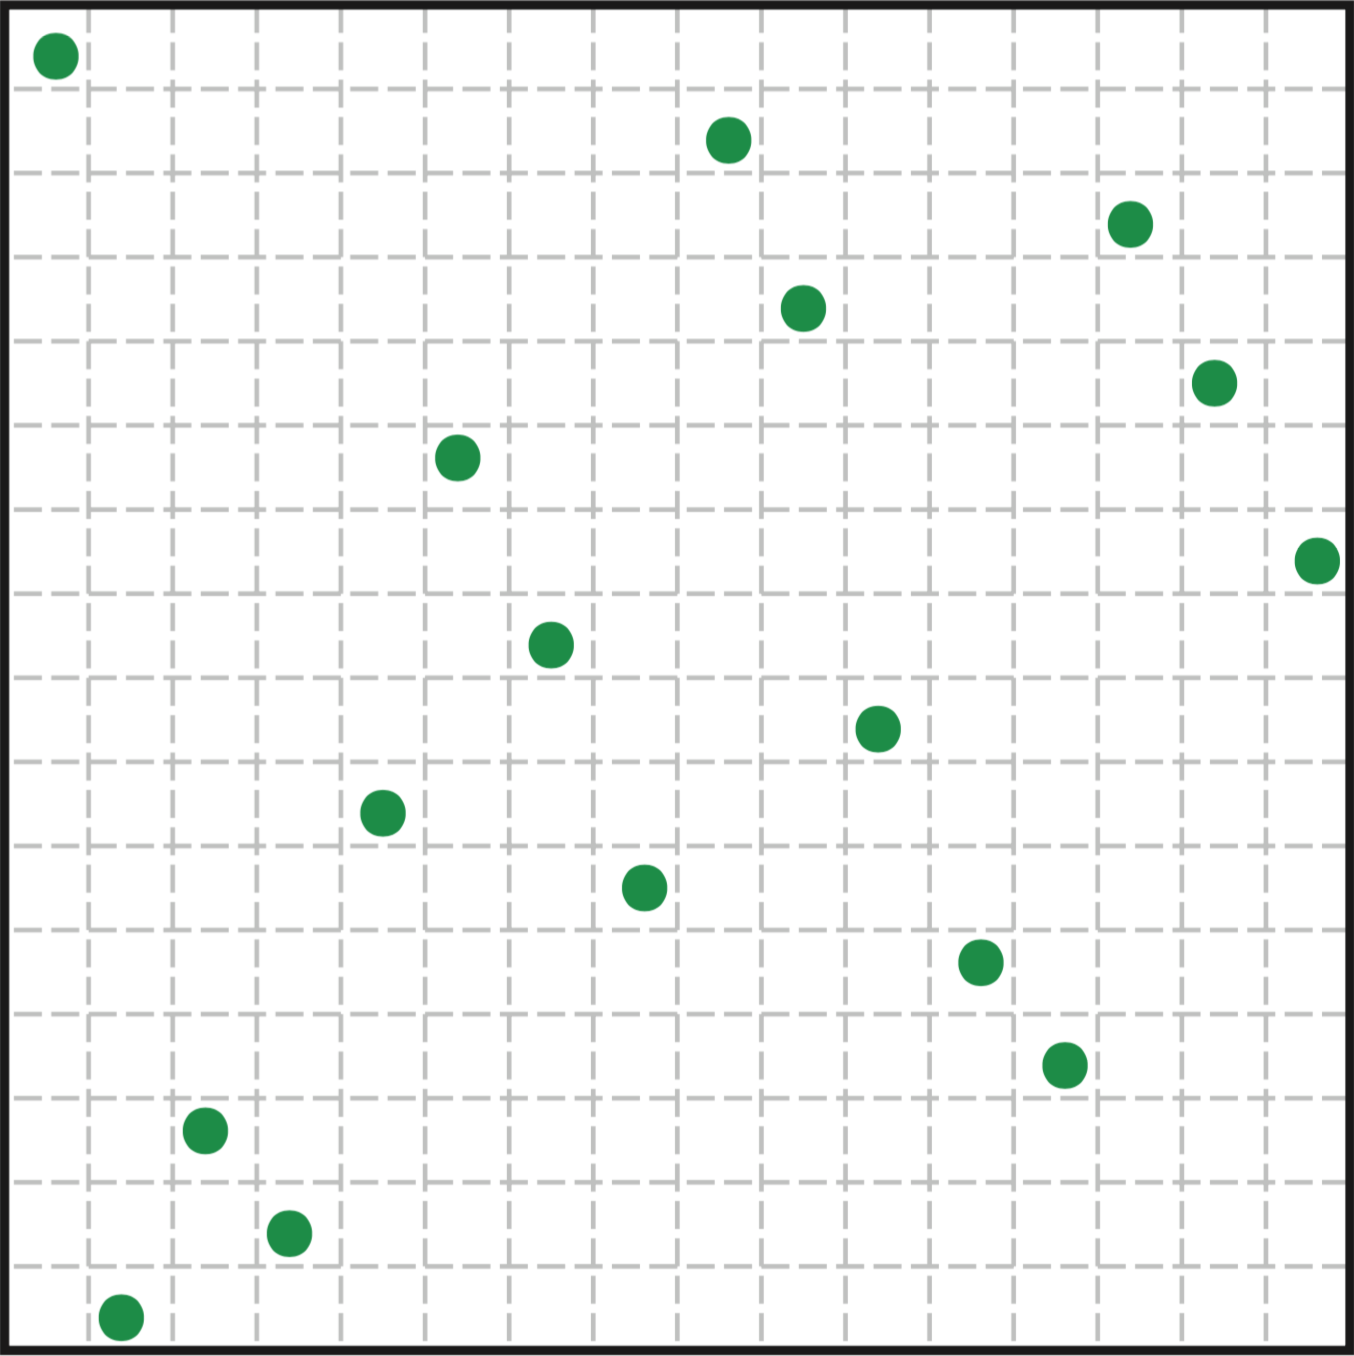
\includegraphics[width=0.3\textwidth]{figures/mc/mc-12-3}
	\caption{在2维的空间中,$N$-rooks算法保证每个行或列不会放置超过两个随机数}
	\label{f:n-rooks}
\end{figure}

分层采样方法的主要缺点是对高维积分是无效的,一般地说,$d$维的定义域空间可能需要$N^d$个阶层划分,针对这个问题,一些变体采样方法被提出,例如$N$-rooks算法保持总的采样数量是固定的,即其与定义域的维度无关。例如,考虑一个2维的函数,使用每个阶层一个采样点的分层采样,一共需要$N^2$个阶层划分;$N$-rooks算法则将这$N$个采样点均匀地分配在各个阶层空间,在这个例子中就是保证每个行和列的组合只包含一个采样点,如图\ref{f:n-rooks}所示,关于$N$-rooks算法,更详细的描述参见Shirley的博士论文\cite{a:PhysicallyBasedLightingCalculationsForComputerGraphics}。

沿着这种改变随机性的思路,拟蒙特卡洛方法则完全去掉随机性,使得随机数完全按照某种固定序列均匀分布来避免丛聚,我们将在下一节讨论拟蒙特卡洛方法。





\subsection{拟蒙特卡洛方法}\label{sec:quasi-monte-carlo}
虽然大数定律证明,当采样数量趋近于无穷的时候,蒙特卡洛估计趋近于期望值的概率为1,但是传统蒙特卡洛方法的收敛速度非常慢,其标准差$\sigma\propto \cfrac{1}{\sqrt{N}}$,即增加4倍的采样数量才能换来2倍的精确度提升。

在上一节中已经证明,分层采样减少了蒙特卡洛估计的方差,这主要是由于阶层的划分减少了随机数导致的丛聚,那么更进一步,我们可不可以采用完全均匀的采样来代替随机分布,使得蒙特卡洛估计的方差进一步降低,收敛速度更快呢?

重新思考蒙特卡洛方法,其随机变量的独立性是指其对应的随机事件之间是不相关的,但是蒙特卡洛方法并没有限制随机数产生的方式,它只要求采样的随机数满足对应的分布。传统的采样方式是使用电脑的伪随机数来进行的,这种随机的特征导致每个随机数并不知道其他随机数的任何信息,所以其分布可能出现丛聚,减慢了收敛速度。所以,理论上如果我们使用确定性(非随机)的方法来产生均匀地分布,那么蒙特卡洛方法的模拟过程不会受到影响,并且收敛速度可以加快。

拟蒙特卡洛方法(Quasi-Monte Carlo method)\mathindex{拟蒙特卡洛方法}{Quasi-Monte Carlo method}就是这样一种方法,它和传统蒙特卡洛方法的唯一不同仅在于随机数产生的方式,拟蒙特卡洛方法使用低差异(low-discrepancy)\mathindex{低差异}{low-discrepancy}序列,这些序列是通过数论方法产生的高度均匀的拟随机数序列,例如霍尔顿序列,索波尔序列等。本节我们将首先讨论均匀性以及拟蒙特卡洛方法的方差,然后介绍几种常见的低差异序列。

设$a$和$c$是$[0,1)^d$区间内的点,对于$a,c$的每个分量$i$都满足$a_i<c_i$,则$[a,c)$可以表示一些点$x$组成的一个盒子区域,对于每个分量$i$这些点满足$a_i\leq x\leq c_i$,我们用$|[a,c)|$表示这个d-维盒子的体积。

设$x_i$是$[0,1)^d$上的随机数,为了分析一个序列的均匀性(uniformity)\mathindex{均匀性}{uniformity}对收敛速度的影响,我们需要一个数值方法来度量一个序列有多么均匀,这个度量称为差异(discrepancy)\myindex{差异}{discrepancy},差异有许多形式,其中的一种称为星差异(star discrepancy)\myindex{星差异}{star discrepancy},它的定义如下:

\begin{equation}
	D^{*}_n=D^{*}_n(x_1,\cdots,x_n)=\sup_{a\in[0,1)^d}\bigg| \cfrac{1}{n}\sum^{n}_{i=1}1_{0\leq x_i<a}-|[0,a)|\bigg|
\end{equation}

\noindent $ \cfrac{1}{n}\sum^{n}_{i=1}1_{0\leq x_i<a}$表示的是盒子内的采样占总采样数量的比例,所以星偏差\footnote{偏差的一般形式定义中盒子$[a,c)$中的$a$和$c$可以取任意值,而不是一个固定在原点的盒子$[0,a)$。}表示的是在所有盒子$[0,a)$中,盒子体积与其盒子内点所占总数比例的差的绝对值的最大值。图\ref{f:mc-discrepancy}展示了这种偏离度的概念,它包含一个固定在原点的盒子$[0,a)\in [0,1)^2$以及一个$n=20$的序列,盒子里面有4个点,所以$(1/n)\sum^{n}_{i=1}1_{0\leq x_i<a}=0.2$,而盒子的体积为$0.6\times 0.25=0.15$,所以其差为$|0.2-0.15|=0.05$,星偏差$D^{*}$是取所有盒子$[0,a)$的最大值。

\begin{figure}
	\sidecaption
	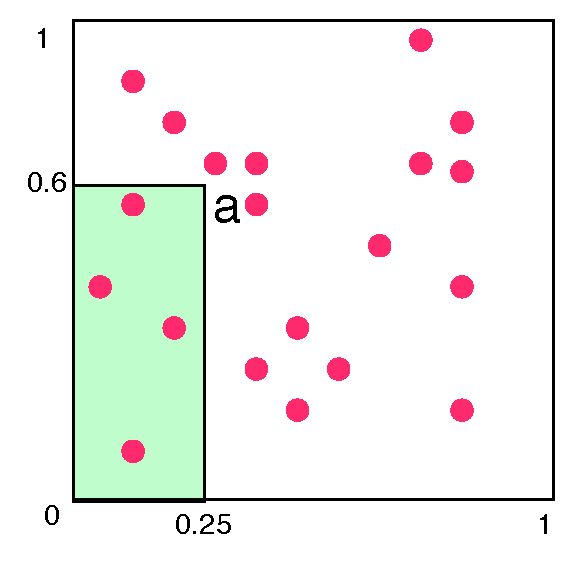
\includegraphics[width=0.3\textwidth]{figures/mc/discrepancy}
	\caption{图为在一个单位正方形内的20个点组成的序列,以及一个固定在原点的盒子,$a=(0.25,0.6)$,盒子的体积为0.15,占据的点的比例为$4/20=0.2$。}
	\label{f:mc-discrepancy}
\end{figure}

有了序列的偏差度的数值定义,我们可以用它来分析序列的均匀性对估计错误程度的影响。拟蒙特卡洛估计的错误被其使用的序列的偏差限定在一个有界区间内,更精确地讲,Koksma–Hlawka不等式(The Koksma–Hlawka inequality)\mathindex{Koksma–Hlawka不等式}{The Koksma–Hlawka inequality}声明拟蒙特卡洛估计的错误\footnote{这里的错误定义和方差是有一点区别的,估计值和期望值之差的绝对值才是估计错误的真实形式,而方差的定义为了避免绝对值带来的麻烦而使用错误平方的期望形式表示。}:

\begin{equation}
	\epsilon=\Bigg| {\rm \int}_{[0,1]^{d}f(\mu){\rm d}\mu}- \cfrac{1}{N}\sum^{N}_{i=1}f(x_i) \Bigg|
\end{equation}

\noindent 被限定在区域:

\begin{equation}
	|\epsilon |\leq V(f)D^{*}_{N}
\end{equation}

\noindent 之内。这里的函数$V(f)$为被积函数$f$的Hardy-Krause方差(Hardy-Krause variation)\mathindex{Hardy-Krause方差}{Hardy-Krause variation},该不等式可以用于展示拟蒙特卡洛估计的错误边界为$O( \cfrac{(\log{N})^{d}}{N})$,而传统蒙特卡洛估计的错误为$O( \cfrac{1}{\sqrt{N}})$。虽然我们只能声明拟蒙特卡洛估计错误的上边界(upper bound)值,但实践上拟蒙特卡洛方法的收敛速度要比理论上快得多,因此一般情况拟蒙特卡洛方法比传统的蒙特卡洛方法的收敛速度要快;此外,从该表达式也可以看出拟蒙特卡洛估计的维数$d$越小,其估计错误越小,收敛速度越快,





\subsubsection{低差异序列}
产生低差异序列的方法和伪随机数序列的方法是完全不同的。产生多维伪随机数序列的间接方法是首先由伪随机数发生器(如系统中的random(u)函数)产生一维随机数序列,然后根据概率论定理,用间接方法(如逆向变换算法,取舍算法等)将一维伪随机数序列转换为多维伪随机数序列;然而拟随机数不是随机的,而是确定的,没有概率统计特性,因此不能像产生多维伪随机数那样的方法工作。

因此我们使用直接方法产生多维拟随机数序列。直接方法即是数论方法,数论方法是基于数论中的一致分布理论,利用数论中关于整数,素数,同余式等知识产生多维拟随机数序列。数论当中有许多方法用于产生低差异序列(low-discrepancy sequence)\mathindex{低差异序列}{low-discrepancy sequence}的方法,本节我们仅讨论比较常用的几种利用倒根函数实现的低差异序列。





\paragraph{倒根函数}
任何一个自然数$i=0,1,2,\cdots,n$可以展开为以$b$为底的正幂次的表达式,即是用$b$进制表示自然数$i$,其中$b$称为基(radix),其展开式为:

\begin{equation}
	i=\sum^{m-1}_{l=0}a_l(i)b^{l}
\end{equation}

\noindent 其中,$a_l(i)$为数字展开式的系数,$m$为数字展开式的项数,$m$决定了$i$在$b$进制下的位数,它允许展开$N=b^{m}$个自然数,例如数字123用10进制表示为$123=3\cdot 10^{0}+2\cdot 10^{1}+1\cdot 10^{2}$。如果我们将展开系数$a_0,a_1,\cdots,a_{m-1}$看成一个$m$维的向量,则该展开式将一个自然数序列转换成了一个多维的向量序列。

有了这个多维向量序列,为了将它转换为$[0,1]^d$空间的向量序列,首先需要将该序列转换为$b$进制的小数形式,这就需要用到倒根函数(radical\footnote{此处radical实际上是取名词radix的形容词形式,因此理解为"根的,基的"意思,和"base"的意思是一致的,因此倒根函数指的是对基进行反向映射,由$b$进制映射回10进制。} inverse function)\mathindex{倒根函数}{radical inverse function},倒根函数表示将该序列转换为以$b$为底的负幂次的表达式,即是$b$进制的小数形式,其定义如下:

\begin{equation}
	\Phi^{-1}_{b,C}(i)=(b^{-1}\cdots b^{-m})\begin{bmatrix}
	 C \begin{pmatrix}
		a_0(i)\\
		\vdots\\
		a_{m-1}(i)
	\end{pmatrix} \end{bmatrix}
\end{equation}

\noindent 其中,$C$是一个生成矩阵(generator matrix)\mathindex{生成矩阵}{generator matrix},生成矩阵通常和底数的选择有关,每个低差异序列算法中的不同点就在于底数$b$和生成矩阵$C$的选择。

有了$b$进制小数形式的多维拟随机向量,最后一步直接将该向量转换为10进制即可,以上的过程就将自然数$0,1,2\cdots,n$一共$n$个数转换为$n$个$[0,1]^{m}$空间上的向量序列,即是我们最终需要的拟随机数序列。以下我们简单介绍两种基于倒根函数生成的低差异序列。




\paragraph{科普特序列}
科普特序列(van der Corput sequence)\mathindex{科普特序列}{van der Corput sequence}是一维的拟随机数序列,其一维底数$b$可取任一素数,$C$为单位矩阵。例如以底数2为例,图\ref{f:mc-corput}列出了16个拟随机数组成的特普特序列,由于$C$为单位矩阵,所以正幂次的2进制形式在转换为负幂次的2进制形式的时候,相当于将每个展开系数的顺序反转,如图\ref{f:mc-corput}中的第二,三列所示。

\begin{figure}
	\sidecaption
	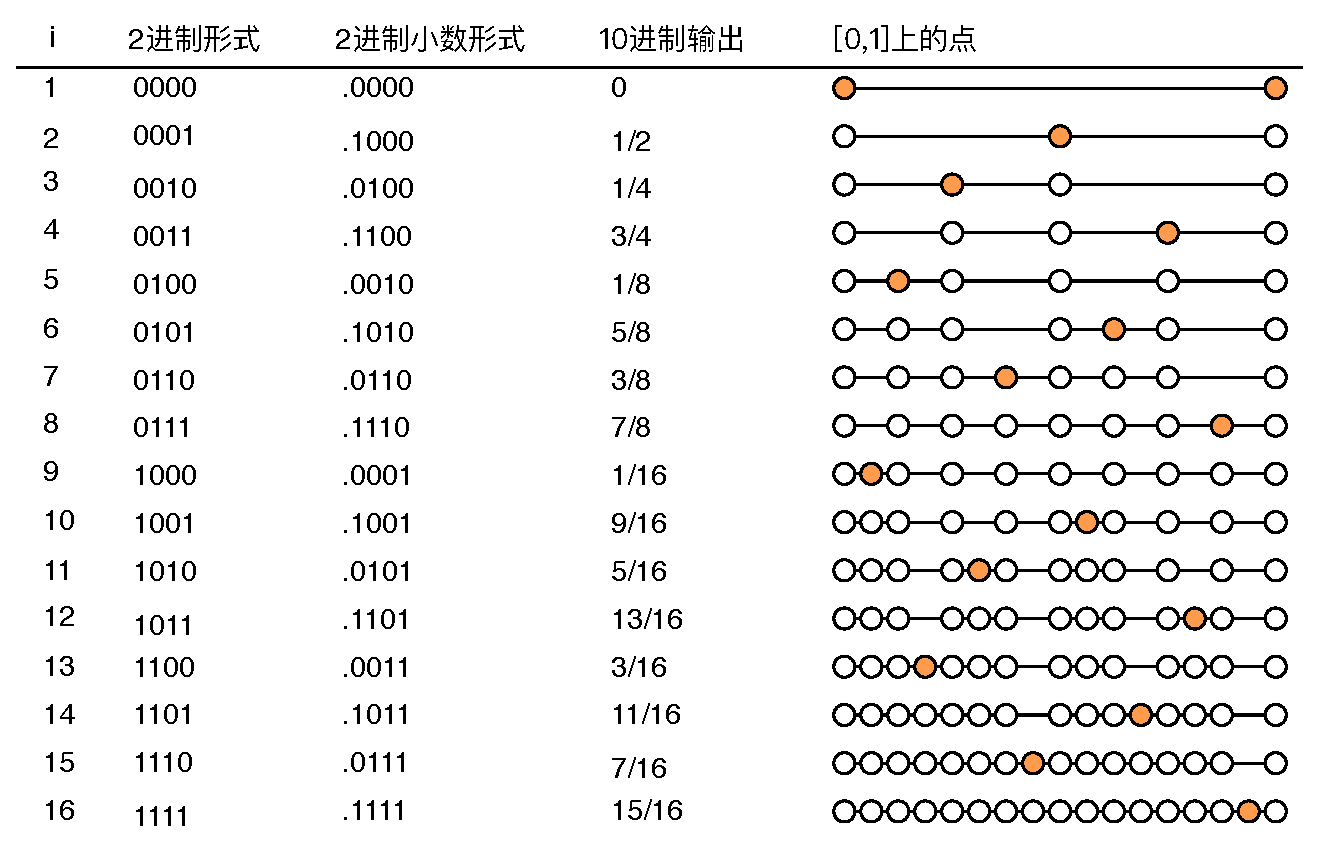
\includegraphics[width=1.0\textwidth]{figures/mc/corput}
\caption{16个拟随机数的一维科普特序列,其中底数$b$为2,$C$为单位矩阵,科普特序列主要就是靠反转二进制形式的各个位的顺序来获得。}
\label{f:mc-corput}
\end{figure}




\paragraph{霍尔顿序列}
另一个常用的低差异序列是霍尔顿序列(Halton sequence)\mathindex{霍尔顿序列}{Halton sequence},霍尔顿序列是科普特序列扩展到高维的一般形式,即是霍尔顿序列的生成矩阵$C$也是单位矩阵,但是霍尔顿序列的底数选择方式不一样,一维的霍尔顿序列就是底数为$2$的科普特序列。

霍尔顿序列的每维有不同的底数,霍尔顿序列第$j$维的底数是第$j$个素数,即维数取值$j=1,2,3,4,5,6,7,8,9,10,\cdots$,对应维数的霍尔顿序列底数取值为$b_j=2,3,5,7,11,13,17,19,23,29,\cdots$,根据数论中的判别素数的相关方法可以得到自然数素数表。

\begin{figure}
\sidecaption
	{\begin{subfigure}[b]{0.32\textwidth}
		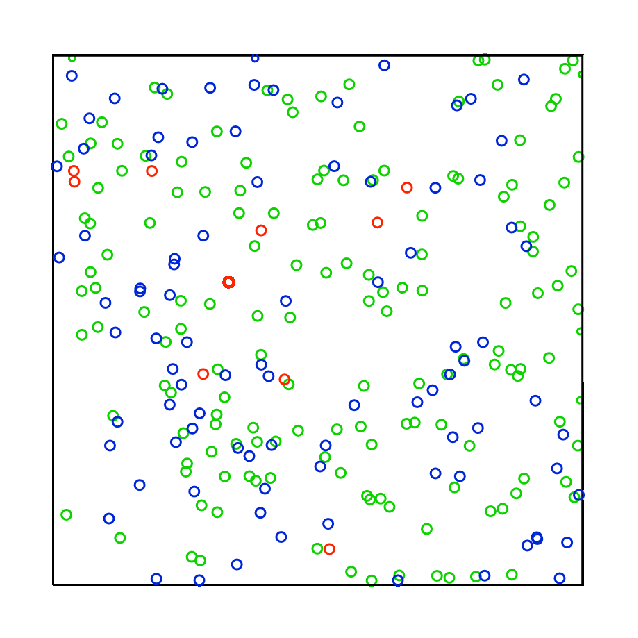
\includegraphics[width=1.\textwidth]{figures/mc/halton-1}
		\caption{伪随机数序列}
	\end{subfigure}
	\begin{subfigure}[b]{0.32\textwidth}
		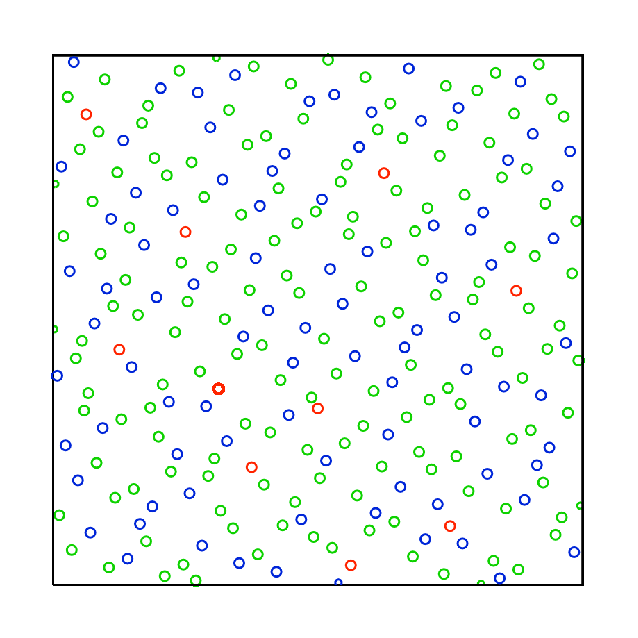
\includegraphics[width=1.\textwidth]{figures/mc/halton-2}
		\caption{霍尔顿序列}
	\end{subfigure}}
	\caption{256个伪随机数序列和开头256个Halton(2,3)序列中随机数的均匀性比较(图片来自Wikipedia) }
	\label{f:mc-halton}
\end{figure}

由于数字展开式$a_l(i)\in \{1,2,\cdots,b_j-1 \}$,而霍尔顿序列的底数随维数增加而增加,所以当维数$j$越高,底数$b$就越大,系数$a_l$个数就越多,计算循环时间越长。此外,由于高维使用的底数是比较大的素数,循环会很长,出现一些空隙结构,所以霍尔顿序列的均匀性在10维以上逐渐变坏,出现丛聚现象,20维以上丛聚就比较明显了,所以并不适合高维的拟随机数序列。

有很多低差异序列用于改善高维霍尔顿序列的退化现象,这里不再详述,相比这些序列,霍尔顿序列的而优势在于生成矩阵$C$为单位矩阵,而其他低差异序列往往有着非常复杂的生成矩阵,计算复杂度大大增加,所以在低维情况下霍尔顿序列几乎是最好的选择。
